% Options for packages loaded elsewhere
% Options for packages loaded elsewhere
\PassOptionsToPackage{unicode}{hyperref}
\PassOptionsToPackage{hyphens}{url}
%
\documentclass[
  12pt,
  letterpaper,
  DIV=11,
  numbers=noendperiod]{scrartcl}
\usepackage{xcolor}
\usepackage[left=1in,right=1in,top=1in,bottom=1in]{geometry}
\usepackage{amsmath,amssymb}
\setcounter{secnumdepth}{5}
\usepackage{iftex}
\ifPDFTeX
  \usepackage[T1]{fontenc}
  \usepackage[utf8]{inputenc}
  \usepackage{textcomp} % provide euro and other symbols
\else % if luatex or xetex
  \usepackage{unicode-math} % this also loads fontspec
  \defaultfontfeatures{Scale=MatchLowercase}
  \defaultfontfeatures[\rmfamily]{Ligatures=TeX,Scale=1}
\fi
\usepackage{lmodern}
\ifPDFTeX\else
  % xetex/luatex font selection
  \setmainfont[ItalicFont=EB Garamond Italic,BoldFont=EB Garamond
SemiBold]{EB Garamond Math}
  \setsansfont[]{EB Garamond SemiBold}
  \setmathfont[]{EB Garamond Math}
\fi
% Use upquote if available, for straight quotes in verbatim environments
\IfFileExists{upquote.sty}{\usepackage{upquote}}{}
\IfFileExists{microtype.sty}{% use microtype if available
  \usepackage[]{microtype}
  \UseMicrotypeSet[protrusion]{basicmath} % disable protrusion for tt fonts
}{}
\usepackage{setspace}
\makeatletter
\@ifundefined{KOMAClassName}{% if non-KOMA class
  \IfFileExists{parskip.sty}{%
    \usepackage{parskip}
  }{% else
    \setlength{\parindent}{0pt}
    \setlength{\parskip}{6pt plus 2pt minus 1pt}}
}{% if KOMA class
  \KOMAoptions{parskip=half}}
\makeatother
% Make \paragraph and \subparagraph free-standing
\makeatletter
\ifx\paragraph\undefined\else
  \let\oldparagraph\paragraph
  \renewcommand{\paragraph}{
    \@ifstar
      \xxxParagraphStar
      \xxxParagraphNoStar
  }
  \newcommand{\xxxParagraphStar}[1]{\oldparagraph*{#1}\mbox{}}
  \newcommand{\xxxParagraphNoStar}[1]{\oldparagraph{#1}\mbox{}}
\fi
\ifx\subparagraph\undefined\else
  \let\oldsubparagraph\subparagraph
  \renewcommand{\subparagraph}{
    \@ifstar
      \xxxSubParagraphStar
      \xxxSubParagraphNoStar
  }
  \newcommand{\xxxSubParagraphStar}[1]{\oldsubparagraph*{#1}\mbox{}}
  \newcommand{\xxxSubParagraphNoStar}[1]{\oldsubparagraph{#1}\mbox{}}
\fi
\makeatother


\usepackage{longtable,booktabs,array}
\usepackage{calc} % for calculating minipage widths
% Correct order of tables after \paragraph or \subparagraph
\usepackage{etoolbox}
\makeatletter
\patchcmd\longtable{\par}{\if@noskipsec\mbox{}\fi\par}{}{}
\makeatother
% Allow footnotes in longtable head/foot
\IfFileExists{footnotehyper.sty}{\usepackage{footnotehyper}}{\usepackage{footnote}}
\makesavenoteenv{longtable}
\usepackage{graphicx}
\makeatletter
\newsavebox\pandoc@box
\newcommand*\pandocbounded[1]{% scales image to fit in text height/width
  \sbox\pandoc@box{#1}%
  \Gscale@div\@tempa{\textheight}{\dimexpr\ht\pandoc@box+\dp\pandoc@box\relax}%
  \Gscale@div\@tempb{\linewidth}{\wd\pandoc@box}%
  \ifdim\@tempb\p@<\@tempa\p@\let\@tempa\@tempb\fi% select the smaller of both
  \ifdim\@tempa\p@<\p@\scalebox{\@tempa}{\usebox\pandoc@box}%
  \else\usebox{\pandoc@box}%
  \fi%
}
% Set default figure placement to htbp
\def\fps@figure{htbp}
\makeatother


% definitions for citeproc citations
\NewDocumentCommand\citeproctext{}{}
\NewDocumentCommand\citeproc{mm}{%
  \begingroup\def\citeproctext{#2}\cite{#1}\endgroup}
\makeatletter
 % allow citations to break across lines
 \let\@cite@ofmt\@firstofone
 % avoid brackets around text for \cite:
 \def\@biblabel#1{}
 \def\@cite#1#2{{#1\if@tempswa , #2\fi}}
\makeatother
\newlength{\cslhangindent}
\setlength{\cslhangindent}{1.5em}
\newlength{\csllabelwidth}
\setlength{\csllabelwidth}{3em}
\newenvironment{CSLReferences}[2] % #1 hanging-indent, #2 entry-spacing
 {\begin{list}{}{%
  \setlength{\itemindent}{0pt}
  \setlength{\leftmargin}{0pt}
  \setlength{\parsep}{0pt}
  % turn on hanging indent if param 1 is 1
  \ifodd #1
   \setlength{\leftmargin}{\cslhangindent}
   \setlength{\itemindent}{-1\cslhangindent}
  \fi
  % set entry spacing
  \setlength{\itemsep}{#2\baselineskip}}}
 {\end{list}}
\usepackage{calc}
\newcommand{\CSLBlock}[1]{\hfill\break\parbox[t]{\linewidth}{\strut\ignorespaces#1\strut}}
\newcommand{\CSLLeftMargin}[1]{\parbox[t]{\csllabelwidth}{\strut#1\strut}}
\newcommand{\CSLRightInline}[1]{\parbox[t]{\linewidth - \csllabelwidth}{\strut#1\strut}}
\newcommand{\CSLIndent}[1]{\hspace{\cslhangindent}#1}



\setlength{\emergencystretch}{3em} % prevent overfull lines

\providecommand{\tightlist}{%
  \setlength{\itemsep}{0pt}\setlength{\parskip}{0pt}}



 


\setlength\heavyrulewidth{0ex}
\setlength\lightrulewidth{0ex}
\KOMAoption{captions}{tableheading}
\makeatletter
\@ifpackageloaded{caption}{}{\usepackage{caption}}
\AtBeginDocument{%
\ifdefined\contentsname
  \renewcommand*\contentsname{Table of contents}
\else
  \newcommand\contentsname{Table of contents}
\fi
\ifdefined\listfigurename
  \renewcommand*\listfigurename{List of Figures}
\else
  \newcommand\listfigurename{List of Figures}
\fi
\ifdefined\listtablename
  \renewcommand*\listtablename{List of Tables}
\else
  \newcommand\listtablename{List of Tables}
\fi
\ifdefined\figurename
  \renewcommand*\figurename{Figure}
\else
  \newcommand\figurename{Figure}
\fi
\ifdefined\tablename
  \renewcommand*\tablename{Table}
\else
  \newcommand\tablename{Table}
\fi
}
\@ifpackageloaded{float}{}{\usepackage{float}}
\floatstyle{ruled}
\@ifundefined{c@chapter}{\newfloat{codelisting}{h}{lop}}{\newfloat{codelisting}{h}{lop}[chapter]}
\floatname{codelisting}{Listing}
\newcommand*\listoflistings{\listof{codelisting}{List of Listings}}
\makeatother
\makeatletter
\makeatother
\makeatletter
\@ifpackageloaded{caption}{}{\usepackage{caption}}
\@ifpackageloaded{subcaption}{}{\usepackage{subcaption}}
\makeatother
\usepackage{bookmark}
\IfFileExists{xurl.sty}{\usepackage{xurl}}{} % add URL line breaks if available
\urlstyle{same}
\hypersetup{
  pdftitle={Age, Period, and Cohort Effects in Philosophy Journal Citations},
  pdfauthor={Anon},
  hidelinks,
  pdfcreator={LaTeX via pandoc}}


\title{Age, Period, and Cohort Effects in Philosophy Journal Citations}
\author{Anon}
\date{2025-02-12}
\begin{document}
\maketitle
\begin{abstract}
There are extremely strong age and period effects in citations in
philosophy journals. The age effect is that citations are concentrated
on articles published two to five years prior. The period effect is that
recent years have seen an explosion in the number of articles published,
and the number of citations per articles, so many articles are getting
more citations per year than they ever had previously. But cohort
effects are trickier to detect. In this note I argue that they exist.
There are more citations to articles from eras of more dramatic change
in philosophy, such as around 1970 and around 2010. And there are fewer
citations to articles from periods of consolidation, especially in the
late 1970s through the 1980s.
\end{abstract}


\setstretch{1.75}
\section{Introduction}\label{sec-introduction}

Before looking at the data, here are two things I believed about
philosophy citations. First, philosophers tend to cite very old papers.
We still regularly teach a number of papers over half a century old in
introductory classes; e.g., Frankfurt
(\citeproc{ref-WOSA1969Y444700002}{1969a}), Thomson
(\citeproc{ref-WOSA1971Y116900003}{1971}), Singer
(\citeproc{ref-WOSA1972Z066400001}{1972}), Lewis
(\citeproc{ref-10.2307_2025310}{1973}). These aren't taught as history
papers, but as early entries into the contemporary philosophical debate.
And, I thought, that's how we cite. Second, the technological changes of
the last quarter century meant that this practice was being slowly
reversed. The spread of electronic communication in the late 20th
century, and then the rise of archives (e.g., Arxiv, SSRN, PhilPapers)
and eventually journals publishing in EarlyView, meant that papers could
now be cited even before they were published, and certainly without the
delays involved in printing and posting journals around the world.

Both of these thoughts were wrong. Historically, philosophy papers have
tended, when they are citing other philosophy papers, to cite very
recent ones. But this tendency is diminishing, not increasing, over
time. I'll offer much more evidence for these claims as we go along, but
to make them plausible, I'll start with two simple graphs.

The data for the graphs come from citation data I downloaded concerning
125,324 papers published from 1955-2024, in one hundred leading
philosophy journals. I focussed on the citations to and from journals in
this dataset. So every citation is from one of these 100 journals
between 1955 and 2024, and to one of these 100 journals between 1955 and
2024. (The details of the journals, including when they start getting
indexed for this dataset, are in Section~\ref{sec-methodology}.) In
total, that gives us YYY citations.

Say the \emph{age} of a citation is the difference between the
publication year of the citing article and the cited article. So if an
article published in 1998 cites an article published in 1985, that's a
13 year old citation.

In Figure~\ref{fig-overall-age} I've plotted the number of citations in
the dataset with each possible age. As you can see, it's very heavily
tilted towards the left-hand edge. It is true that people still cite
Frankfurt (\citeproc{ref-Frankfurt1969}{1969b}). Indeed, it's one of the
most cited papers in the last ten years. But it's just one paper; the
bulk of citations are to recently published papers which, if history is
any guide, will soon stop collecting citations.

\begin{figure}

\centering{

\pandocbounded{\includegraphics[keepaspectratio]{apc-2025-50_files/figure-pdf/fig-overall-age-1.pdf}}

}

\caption{\label{fig-overall-age}Number of citations with each age.}

\end{figure}%

In Figure~\ref{fig-overall-median-mode} I've plotted the median and mode
age of citations in each year from 1980 onwards. Before that the numbers
are even lower, but since I'm only looking at citations to articles
published after 1955 (or later if Web of Science started indexing the
journal later than that), this is arguably an artifact of how I'm
collecting the data. From 1980 onwards, however, there are many older
articles that could be, but are not, getting cited. The upwards trends
in both graphs look like a real change in citation practices, and not in
the direction I antecedently expected.

\begin{figure}

\begin{minipage}{\linewidth}

\centering{

\pandocbounded{\includegraphics[keepaspectratio]{apc-2025-50_files/figure-pdf/fig-overall-median-mode-1.pdf}}

}

\subcaption{\label{fig-overall-median-mode-1}Median}

\end{minipage}%
\newline
\begin{minipage}{\linewidth}

\centering{

\pandocbounded{\includegraphics[keepaspectratio]{apc-2025-50_files/figure-pdf/fig-overall-median-mode-2.pdf}}

}

\subcaption{\label{fig-overall-median-mode-2}Mode}

\end{minipage}%

\caption{\label{fig-overall-median-mode}Summary statistics for outbound
citations each year 1970-2024.}

\end{figure}%

There is a third surprise in the data, but it's a little more equivocal,
and I'm not sure what to make of it. The 2010s seemed like, and to be
honest still seem like, something of a golden age for philosophy. In
metaphysics we saw the biggest paradigm shift in many years, away from
modality and towards grounding. We saw the growth of important fields of
social philosophy, including social epistemology, social metaphysics,
and social philosophy of language. Though there were some earlier papers
that have become important to the latter two fields (e.g., Haslanger
(\citeproc{ref-Haslanger2000}{2000b}), and Langton
(\citeproc{ref-Langton1993}{1993})), it would have been a stretch to
even call them `fields' before 2010. Social epistemology was always a
bit bigger, and you could point to earlier field defining work by, e.g.,
Jennifer Lackey (\citeproc{ref-Lackey2008}{2008}) and Adam Elga
(\citeproc{ref-Elga2007}{2007a}). But it grew phenomenally in the 2010s.
I'd predicted that would show up in higher citations to work in the
2010s, as these changes were consolidated. The data are a bit messy, and
it would be good to have much more data, but this does not look to have
happened. There isn't as neat a graph for this, however, and we'll
return to this point at the end.

\section{Age, Period, and Cohort}\label{sec-apc-described}

To help understand the citation patterns, I'll borrow some terminology
that's common in both sociology and medicine. Imagine that we see, in
the historical record, some interesting patterns among teenagers in the
late 1960s, and we're wondering what could explain the pattern. Two
types of pattern spring immediately to mind, along with ways to test
them.

First, the behaviour could be explained by the fact the people involved
are teenagers. If so, it is an \textbf{age effect}. The natural way to
test this is to see if similar patterns show up with teenagers at
different times.

Second, the behaviour could be explained by the fact that it was the
1960s, and lots of striking things happened in the 1960s. If so, it is a
\textbf{period effect}. The natural way to test this is to see if the
same pattern shows up with non-teenagers in the 1960s.

There is an important third kind of explanation. The people involved are
born in the early 1950s, so they are part of the post-war baby boom.
Colloquially, they are boomers. Maybe that could explain the pattern we
see. If so, it is a \textbf{cohort effect}. The natural way to test this
is to see if the same pattern shows up if we look at the same people in
other stages of their life.

It's easy to overlook the importance of cohort effects. Sometimes they
simply look like age effects. Ghitza, Gelman, and Auerbach
(\citeproc{ref-GhitzaEtAl2023}{2023}) argue that many hypotheses about
age effects on voting, e.g., that older people are more naturally
conservative, are really just cohort effects. Bump
(\citeproc{ref-Bump2023}{2023}) argues that understanding the
distinctive role the boomers in particular play is crucial for
understanding many aspects of modern American life.

There are mathematical reasons that it is hard to tease these effects
apart too. Many statistical techniques for separating out influences
start to fall apart when there are linear correlations between
combinations of variables. In this case there is as tight a correlation
as is possible. By definition, cohort plus age equals period. There are
some things you can do to get around this problem - see Keyes et al.
(\citeproc{ref-KeyesEtAl2010}{2010}) for a useful survey of some of the
options - but it remains a challenge.

Even conceptually, it is hard to separate out these three effects in
cases where there is evidence that the strength of the effects changes
over time. As I noted at the start, the natural way to test hypotheses
about which effect is strongest involve looking at other times. That
works well when the age effects are constant. When they are not (and
they might not be here), it is harder.

For most of our story, however, it helps just to have these three
effects in mind. Using them, we can summarise the data reasonably
quickly.

\begin{itemize}
\tightlist
\item
  The age effect is that articles get cited most when they are two to
  five years old, as shown in Figure~\ref{fig-overall-age}.
\item
  The period effect is that there are many more citations in recent
  years than in earlier years. This is in part because the number of
  articles published in these journals has been growing, and in part
  because the number of citations per article grew substantially over
  the 2000s and 2010s, and exploded in the 2020s.
\item
  The cohort effect is that articles from the 1970s and 2000s get cited
  more than you'd expect given these age and period effects, articles
  from before the late-1960s get barely cited at all, and articles from
  1980 through the mid-1990s also get cited considerably less than
  articles either side of that period. I'll offer some speculations at
  the end of the paper about the philosophical causes of, and
  consequences of, these cohort effects.
\end{itemize}

As I mentioned above, I'll go over the methodology in detail in
Section~\ref{sec-methodology}. But there is one point that is important
to note before we start. I'm using data from Web of Science, and they
typically don't start indexing journals until well after the journal is
established. So the first year of citation data I have for
\emph{Analysis} is 1975. Crucially, that means that ``Is Knowledge
Justified True Belief?'' (\citeproc{ref-Gettier1963}{Gettier 1963}) is
not included in this study. If it were, and in general if I had the data
from \emph{Analysis} to work from, some of the results about the early
1960s would look less dramatic, though as far as I can tell, the
direction of the results wouldn't change.

\section{Period Effects}\label{sec-period}

Those 509004 citations are not distributed evenly over time. Instead,
they grow rapidly. At the start, in 1956, there are only 5 citations.
That's not too surprising; without the ability to cite preprints, there
aren't going to be many citations of articles that have come out that
year. By 2024, there are 38507. In Figure~\ref{fig-citationsperyear}, I
show how these grew; the striking thing to me is XXXXXXXXXXXXXXX.

\begin{figure}

\centering{

\pandocbounded{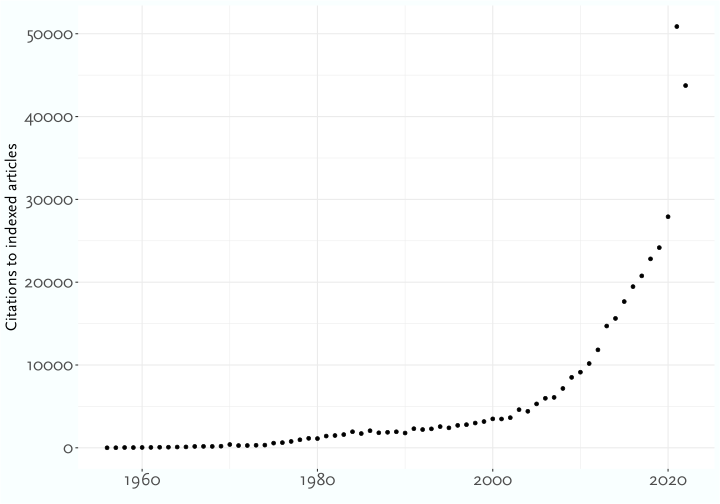
\includegraphics[keepaspectratio]{apc-2025-50_files/figure-pdf/fig-citationsperyear-1.pdf}}

}

\caption{\label{fig-citationsperyear}The number of citations in the
dataset made each year.}

\end{figure}%

What explains this dramatic growth? Part of the explanation is that more
articles are being published, and more articles are being indexed.
Figure~\ref{fig-articlesperyear} shows how many articles are in the
dataset each year.

\begin{figure}

\centering{

\pandocbounded{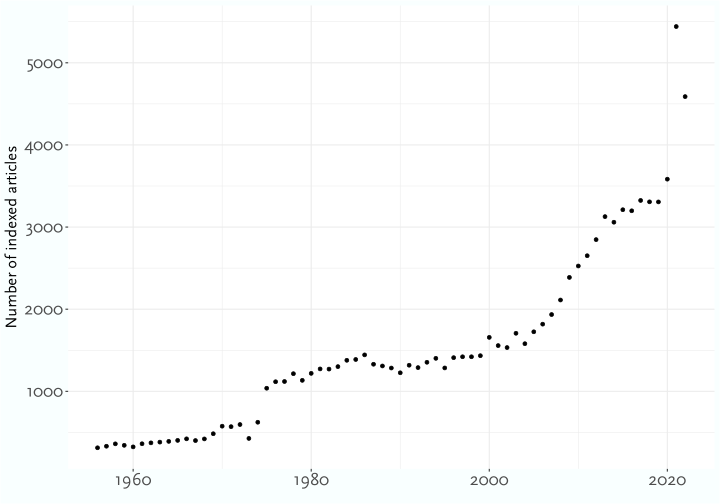
\includegraphics[keepaspectratio]{apc-2025-50_files/figure-pdf/fig-articlesperyear-1.pdf}}

}

\caption{\label{fig-articlesperyear}The number of articles in the
dataset published each year.}

\end{figure}%

That explains some of the growth, but not all of it. The curve in
Figure~\ref{fig-articlesperyear} is not nearly as steep as the curve in
Figure~\ref{fig-citationsperyear}. The number of (indexed) citations per
article is also rising. In Figure~\ref{fig-outboundcitations} I've
plotted the average number of citations to other articles in the dataset
each year.

\begin{figure}

\centering{

\pandocbounded{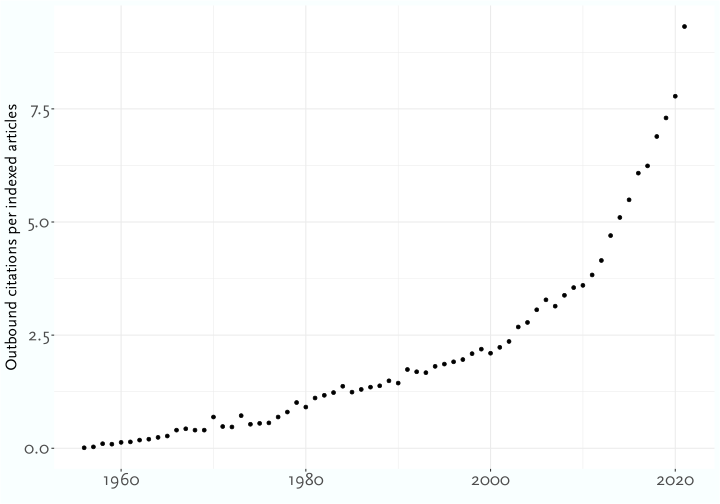
\includegraphics[keepaspectratio]{apc-2025-50_files/figure-pdf/fig-outboundcitations-1.pdf}}

}

\caption{\label{fig-outboundcitations}The average number of citations to
indexed articles each year.}

\end{figure}%

There are a few possible explanations for the shape of this graph.

At the left-hand edge, there are obvious boundary effects. Since we're
only counting citations to articles published since 1956, it isn't
surprising that there aren't very many of them per article in the 1950s.
Since articles rarely get unpublished, there are more articles available
to cite every year.

That can't explain the massive jumps we see at the right hand edge of
Figure~\ref{fig-outboundcitations}. The jump there looks like the
convergence of two cultural trends. One is a trend simply to greater
numbers of citations. The most casual perusal of journals will confirm
that trend. The other is a trend to greater citations of journals
themselves, as opposed to books or edited volumes.

A sharp jump like this is a warning sign that there is something wrong
with the data. It's impractical to cross-check every entry, but those I
have checked look correct. The change seems led by the most prestigious
journals. For each journal I calculated the average number of outbound
citations (to these hundred journal) for both the 2010s, and the first
two years of the 2020s. The ten journals with the largest increase
between the decades are shown in Table~\ref{tbl-large-growth}.

\begin{longtable}[]{@{}
  >{\raggedright\arraybackslash}p{(\linewidth - 6\tabcolsep) * \real{0.5694}}
  >{\raggedleft\arraybackslash}p{(\linewidth - 6\tabcolsep) * \real{0.1389}}
  >{\raggedleft\arraybackslash}p{(\linewidth - 6\tabcolsep) * \real{0.1389}}
  >{\raggedleft\arraybackslash}p{(\linewidth - 6\tabcolsep) * \real{0.1528}}@{}}

\caption{\label{tbl-large-growth}Mean outbound citations for some
journals over the last two decades.}

\tabularnewline

\toprule\noalign{}
\begin{minipage}[b]{\linewidth}\raggedright
Journal
\end{minipage} & \begin{minipage}[b]{\linewidth}\raggedleft
2010-2019
\end{minipage} & \begin{minipage}[b]{\linewidth}\raggedleft
2020-2024
\end{minipage} & \begin{minipage}[b]{\linewidth}\raggedleft
Difference
\end{minipage} \\
\midrule\noalign{}
\endhead
\bottomrule\noalign{}
\endlastfoot
Philosophical Review & 14.8 & 26.3 & 11.5 \\
Philosophical Perspectives & 11.3 & 19.2 & 7.9 \\
Noûs & 11.5 & 18.4 & 6.9 \\
Philosophy and Phenomenological Research & 9.6 & 15.8 & 6.2 \\
Philosophical Studies & 9.0 & 14.6 & 5.6 \\
Journal of Philosophy & 9.0 & 14.5 & 5.6 \\
Philosophy & 4.0 & 8.9 & 4.9 \\
Episteme & 8.1 & 12.9 & 4.9 \\
Philosophical Quarterly & 8.8 & 13.6 & 4.7 \\
Philosophy Compass & 11.2 & 15.9 & 4.7 \\

\end{longtable}

Since \emph{Philosophical Review} only publishes 10 to 12 articles per
year, it is not surprising that it shows the most variation on this
list. Still, the change in the 2010s isn't only small sample size
variation.

Although the number of citations is going up, the number of articles
available to be cited is also going up. Say an article is
\emph{available} if it is published in a year iff it is published in or
before that year. That's not quite right in either direction; some
articles are cited before publication, some articles that come out in
December aren't in any real sense available to be cited in January. But
it's close enough. Say an article is from a year that is
\emph{typically} cited iff it is between 3 and 10 years before the
citing year. This notion will play a big role in Section~\ref{sec-age};
I'm going to use these as a way of getting something like a base rate
for citations in a given year. Using these definitions,
Figure~\ref{fig-articlecounts} shows how many articles are available to
be cited each year, and are from years that are typically cited.

\begin{figure}

\begin{minipage}{\linewidth}

\centering{

\pandocbounded{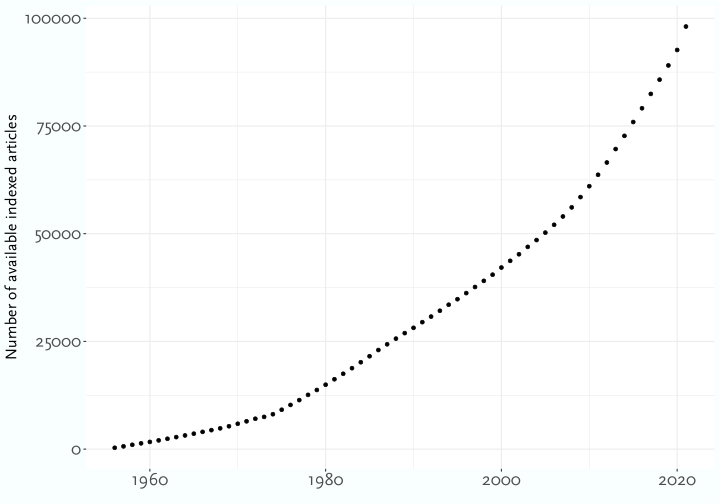
\includegraphics[keepaspectratio]{apc-2025-50_files/figure-pdf/fig-articlecounts-1.pdf}}

}

\subcaption{\label{fig-articlecounts-1}Available articles}

\end{minipage}%
\newline
\begin{minipage}{\linewidth}

\centering{

\pandocbounded{\includegraphics[keepaspectratio]{apc-2025-50_files/figure-pdf/fig-articlecounts-2.pdf}}

}

\subcaption{\label{fig-articlecounts-2}Typically cited articles}

\end{minipage}%

\caption{\label{fig-articlecounts}Article counts.}

\end{figure}%

In Figure~\ref{fig-citationcounts}, I've shown how often, in each year,
the available articles, and the `typical' articles are cited. The
`available' graph is obviously similar to
Figure~\ref{fig-citationsperyear}; under 1\% of citations are to
articles published in future years. One thing that will be useful in
Section~\ref{sec-age} is that the graphs in
Figure~\ref{fig-citationcounts} have a similar shape.

\begin{figure}

\begin{minipage}{\linewidth}

\centering{

\pandocbounded{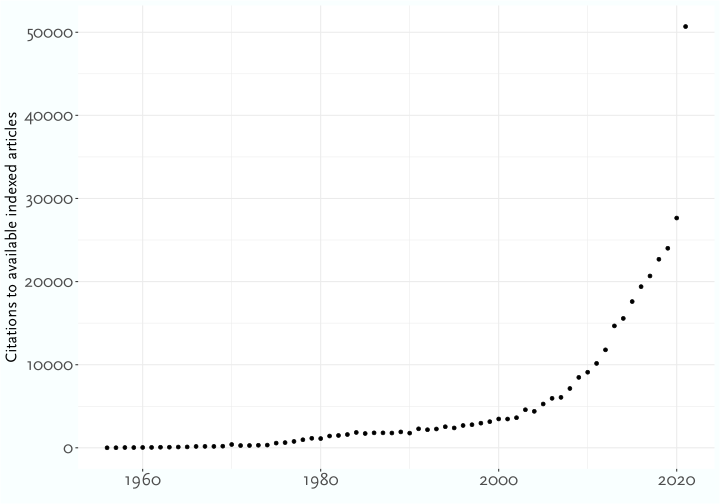
\includegraphics[keepaspectratio]{apc-2025-50_files/figure-pdf/fig-citationcounts-1.pdf}}

}

\subcaption{\label{fig-citationcounts-1}Citations to available articles}

\end{minipage}%
\newline
\begin{minipage}{\linewidth}

\centering{

\pandocbounded{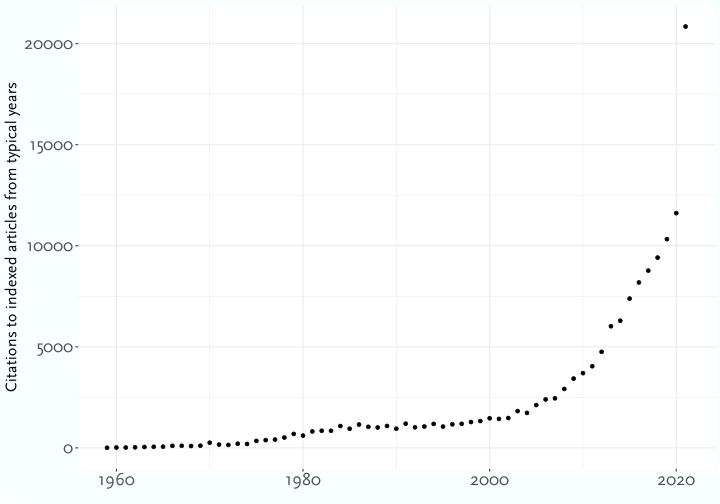
\includegraphics[keepaspectratio]{apc-2025-50_files/figure-pdf/fig-citationcounts-2.pdf}}

}

\subcaption{\label{fig-citationcounts-2}Citations to typical articles}

\end{minipage}%

\caption{\label{fig-citationcounts}Citation counts.}

\end{figure}%

Putting all these together we can work out how often, on average,
available articles, and typical articles, are cited in each year. The
results are in Figure~\ref{fig-citationrate}.

\begin{figure}

\begin{minipage}{\linewidth}

\centering{

\pandocbounded{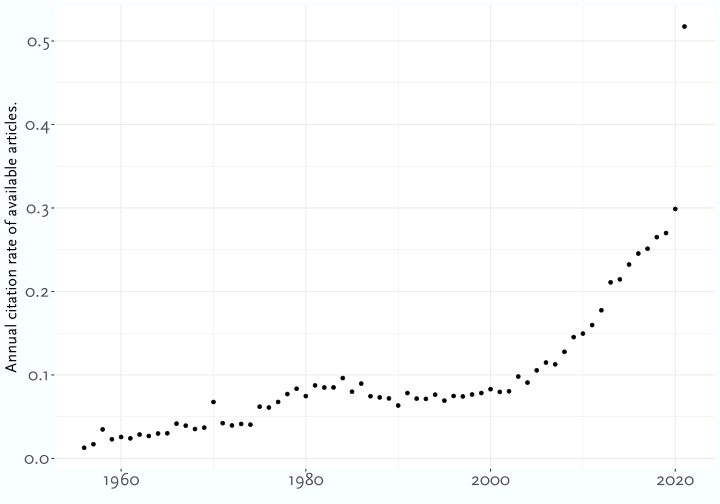
\includegraphics[keepaspectratio]{apc-2025-50_files/figure-pdf/fig-citationrate-1.pdf}}

}

\subcaption{\label{fig-citationrate-1}Available articles}

\end{minipage}%
\newline
\begin{minipage}{\linewidth}

\centering{

\pandocbounded{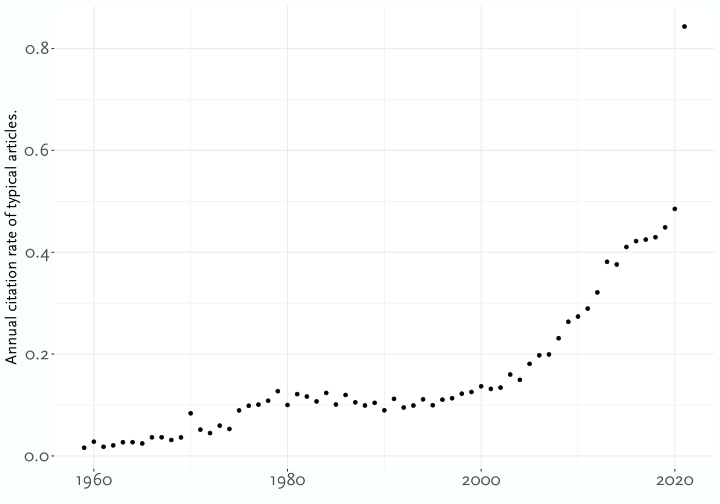
\includegraphics[keepaspectratio]{apc-2025-50_files/figure-pdf/fig-citationrate-2.pdf}}

}

\subcaption{\label{fig-citationrate-2}Typical articles}

\end{minipage}%

\caption{\label{fig-citationrate}Mean annual citations to different
article kinds.}

\end{figure}%

Three things stand out about Figure~\ref{fig-citationrate}. One is that
the two graphs have pretty similar shapes. Using citations from 3 to 10
years prior to the citing year is a pretty good proxy for all citations,
and it turns out to be stable in other ways. A second is that both
graphs are fairly flat for a long time. Between the mid 1970s and early
2000s they bounce around without moving much. Then they take off, and go
through the roof in 2021.\footnote{XXXXX: Check how this looks with new
  data.} The other thing is that these are low numbers. For most of this
study, an arbitrary article in one of these hundred journals was cited
in one of those journals once a \emph{decade}. Actually, since citation
rates are extremely long-tailed, and mean rates are well above medians,
that somewhat overstates how often the `average article' was being
cited. Frequent citation is very much not the norm.\footnote{In the long
  run the average number of times an article is cited equals the average
  number of citations per article. So it shouldn't be too surprising
  that most article have just a handful of citations in philosophy
  journals.}

The various period effects are substantial; to get an reliable picture
of the trends in citation patterns, we're going to have to allow for
them. The project here is to use citation data as a proxy for
philosophical influence. It is, of course, a deeply imperfect proxy. But
it is better than most other proxies; it is certainly better than going
off of vibes, or of what one's friends are talking about.\footnote{In
  North America, placement on graduate syllabi might be an even better
  proxy, but that data is hard to collect, and we'd need a different
  measure for other countries.} If we're going to use citations this way
though, we need to think about how to take into account the changes
shown in Figure~\ref{fig-citationsperyear}. I'm going to offer a
proposal in terms of typical articles; to a first approximation, I'll
measure an article's influence in a period by the ratio of how often it
is cited to how often a typical article is cited. This is a little
arbitrary, but I think it gets things at least roughly right. At the
very least, it avoids the problems with three other natural proposals
that I'll now present, and probably anything that avoids these problems
will be fairly similar.

Start with the non-proposal of just using citations per year as a
measure of influence. Simply eyeballing
Figure~\ref{fig-citationsperyear} makes that a little implausible; there
would be so much more influence now. It also has some implausible
particular consequences. Tyler Burge's ``Individualism and Psychology''
(\citeproc{ref-WOSA1986AYX3200001}{Burge 1986}) was the fourth most
cited paper of the 1990s, and if anything that understates its
influence.\footnote{XXXXXX - old text I have to confirm: In the 1990s
  (in these 100 journals) it had 68 citations, so 6.8 per year. In 2021,
  it had 7 citations, so slightly more per year. Now Burge's paper is
  still influential, and it connects in interesting ways to the social
  turn in philosophy that I'll discuss below, but it's implausible to
  say that it was more influential in 2021 than it was in the 1990s.
  When there are so many articles published, and a much lower bar to
  citation, seven citations a year doesn't signify as much influence.}

A natural second proposal then is to measure what proportion of the
year's citations any particular article has. By this measure,
``Individualism and Psychology'' was about twenty times as influential
in the 1990s as in 2021, which isn't obviously false.\footnote{To be
  clear, the database contains about twice as many citations in 2021 as
  in the whole of the 1990s.} Other cases, however, suggest this is too
much of a correction. It's true that there are more citations now than
there used to be. There are also more articles for these citations to be
shared between. Holding fixed how influential an article is, you'd
expect it to have a lower share of the citations when there are several
times more articles available to be cited.

Again, it's easiest to see this with some examples. In
Table~\ref{tbl-comp-cite-rate}, I've shown the five most cited articles
for the 1990s (on the top), and for 2021 (on the bottom). I've also
shown how often each is cited per 1000 citations, i.e., the proportion
of citations each article gets. And I've extended the first table to
make it easier to compare the scales.

\begin{table}

\caption{\label{tbl-comp-cite-rate}Most cited articles in the 1990s, and
in 2021.}

\begin{minipage}{\linewidth}

\subcaption{\label{tbl-comp-cite-rate-1}1990s}

\centering{

\begin{tabular}{rlrr}
\toprule
Rank & Article & Citations & Citations per 1000\\
\midrule
1 & Frankfurt (\citeproc{ref-10.2307_2024717}{1971}) & 82 & 2.69\\
2 & Kim (\citeproc{ref-WOSA1984TV24600001}{1984}) & 72 & 2.36\\
3 & Nagel (\citeproc{ref-WOSA1974U469700001}{1974}) & 69 & 2.26\\
4 & Burge (\citeproc{ref-WOSA1986AYX3200001}{1986}) & 68 & 2.23\\
 & \ldots{} &  & \\
10 & Kripke (\citeproc{ref-WOSA1975BF60000005}{1975}) & 52 & 1.70\\
 & \ldots{} &  & \\
34 & Hull (\citeproc{ref-WOSA1978FR68900001}{1978}) & 33 & 1.08\\
35 & Lewis (\citeproc{ref-WOSA1979JB14500003}{1979a}) & 33 & 1.08\\
36 & van Fraassen
(\citeproc{ref-WOSA1984SS95000001}{1984}) & 33 & 1.08\\
\bottomrule
\end{tabular}

}

\end{minipage}%
\newline
\begin{minipage}{\linewidth}

\subcaption{\label{tbl-comp-cite-rate-2}2021}

\centering{

\begin{tabular}{rlrr}
\toprule
Rank & Article & Citations & Citations per 1000\\
\midrule
1 & Lewis (\citeproc{ref-WOSA1983RR51600001}{1983}) & 78 & 1.56\\
2 & Machamer, Darden, and Craver
(\citeproc{ref-WOS000087305900001}{2000}) & 54 & 1.08\\
3 & Lewis (\citeproc{ref-10.2307_2025310}{1973}) & 53 & 1.06\\
4 & Clark and Chalmers
(\citeproc{ref-WOS000073222300002}{1998}) & 51 & 1.02\\
5 & Schaffer (\citeproc{ref-WOS000272855000002}{2010}) & 51 & 1.02\\
6 & Elga (\citeproc{ref-WOS000249103800005}{2007b}) & 45 & 0.90\\
7 & Haslanger (\citeproc{ref-WOS000085841900002}{2000a}) & 43 & 0.86\\
8 & Davidson (\citeproc{ref-WOSA1963CEU0700001}{1963}) & 43 & 0.86\\
9 & Nagel (\citeproc{ref-WOSA1974U469700001}{1974}) & 43 & 0.86\\
10 & Lewis (\citeproc{ref-WOSA1979HJ57600007}{1979b}) & 42 & 0.84\\
\bottomrule
\end{tabular}

}

\end{minipage}%

\end{table}%

As influential as ``A Matter of Individuality'', ``Counterfactual
Dependence and Time's Arrow'', and ``Belief and the Will'' were in the
1990s, I don't think they were more influential than all but one article
was in 2021. Haslanger's article became a foundational text for one of
the biggest fields in philosophy: social metaphysics. A measure of
influence that puts it behind how influential 36 articles were in the
1990s seems wrong, and the intuitive reasoning about sharing citations
around suggests why it is wrong.

A natural next move is to scale the citations not to all citations, but
to the average number of citations that available, i.e., already
published, articles get. This would solve the problem I just presented
in a simple way. Having 1 cite per 1000 citations means a lot more when
there are 100,000 articles that could have received that citation than
when there are 10,000 such articles.

Again, this is an overcorrection. In theory, any article already
published could be cited. In practice, long forgotten articles are long
forgotten and hence not cited, and most articles are long forgotten.
It's true that in 2021 articles have to `share' citation space with more
other articles. But in practice that normally means they share the space
with other \emph{recently published} articles.

We can sort of see this by redoing the calculation from
Table~\ref{tbl-comp-cite-rate}, instead using the ratio of citations
this article receives to citations the average available article
receives.\footnote{On the first part of Table~\ref{tbl-comp-cite-ratio},
  I calculated this ratio for each year, and then displayed the average
  over the decade.} I've done this in Table~\ref{tbl-comp-cite-ratio}.
First, I've shown the articles that, across the 1990s, had the highest
average ratio of citations they received to citations the average
available article received, and second, I did the same calculation for
2021.

\begin{table}

\caption{\label{tbl-comp-cite-ratio}Most cited articles in the 1990s
compared to average citations, and in 2021.}

\begin{minipage}{\linewidth}

\subcaption{\label{tbl-comp-cite-ratio-1}1990s}

\centering{

\begin{tabular}{rlr}
\toprule
Rank & Article & Ratio\\
\midrule
1 & Frankfurt (\citeproc{ref-10.2307_2024717}{1971}) & 101.78\\
2 & Kim (\citeproc{ref-WOSA1984TV24600001}{1984}) & 89.60\\
3 & Nagel (\citeproc{ref-WOSA1974U469700001}{1974}) & 85.39\\
4 & Burge (\citeproc{ref-WOSA1986AYX3200001}{1986}) & 84.42\\
5 & Perry (\citeproc{ref-WOSA1979HE39600001}{1979}) & 77.75\\
6 & Lewis (\citeproc{ref-WOSA1983RR51600001}{1983}) & 75.45\\
7 & Jackson (\citeproc{ref-WOSA1982NH65300003}{1982}) & 71.08\\
8 & Kripke (\citeproc{ref-WOSA1975BF60000005}{1975}) & 65.43\\
9 & Cummins (\citeproc{ref-WOSA1975BF60100001}{1975}) & 64.89\\
10 & Lewis (\citeproc{ref-10.2307_2025310}{1973}) & 64.51\\
\bottomrule
\end{tabular}

}

\end{minipage}%
\newline
\begin{minipage}{\linewidth}

\subcaption{\label{tbl-comp-cite-ratio-2}2021}

\centering{

\begin{tabular}{rlr}
\toprule
Rank & Article & Ratio\\
\midrule
1 & Lewis (\citeproc{ref-WOSA1983RR51600001}{1983}) & 174.97\\
2 & Machamer, Darden, and Craver
(\citeproc{ref-WOS000087305900001}{2000}) & 121.13\\
3 & Lewis (\citeproc{ref-10.2307_2025310}{1973}) & 118.89\\
4 & Clark and Chalmers
(\citeproc{ref-WOS000073222300002}{1998}) & 114.40\\
5 & Schaffer (\citeproc{ref-WOS000272855000002}{2010}) & 114.40\\
6 & Elga (\citeproc{ref-WOS000249103800005}{2007b}) & 100.94\\
 & \ldots{} & \\
12 & Hawthorne and Stanley
(\citeproc{ref-WOS000262624000001}{2008}) & 87.49\\
 & \ldots{} & \\
35 & Goldman (\citeproc{ref-WOS000170434600004}{2001}) & 65.05\\
\bottomrule
\end{tabular}

}

\end{minipage}%

\end{table}%

None of the pairwise comparisons here seem obviously absurd. Was ``To be
F is to be G'' more influential in 2021 than ``Causation'' was in the
1990s? I wouldn't have thought so, though it's not as clear as in the
previous set of comparisons. What is clear is that the numbers in the
second table in Table~\ref{tbl-comp-cite-ratio} are considerably higher
than the first table, especially at the very top end. That suggests that
the intuition that including so many articles from long ago in the
comparison class was a mistake, and it has systematically increased the
measure we're using for later years in implausible ways.

So what I've settled on is using the ratio of how often this article is
cited in a year, to how often a \emph{typical} article is cited that
year. By `typical' I mean an article three to ten years old; as we'll
see in Section~\ref{sec-age}, those are the typical ages of cited
articles. That deals with the intuitive problems of the previous
measures, and it gets the results roughly right. In
Table~\ref{tbl-comp-cite-ratio-typical}, I'll do one last comparison
between the 1990s and 2021 to make the point.

\begin{table}

\caption{\label{tbl-comp-cite-ratio-typical}Most cited articles in the
1990s compared to typical citations, and in 2021.}

\begin{minipage}{\linewidth}

\subcaption{\label{tbl-comp-cite-ratio-typical-1}1990s}

\centering{

\begin{tabular}{rlr}
\toprule
Rank & Article & Ratio\\
\midrule
1 & Frankfurt (\citeproc{ref-10.2307_2024717}{1971}) & 71.26\\
2 & Kim (\citeproc{ref-WOSA1984TV24600001}{1984}) & 63.49\\
3 & Nagel (\citeproc{ref-WOSA1974U469700001}{1974}) & 59.55\\
4 & Burge (\citeproc{ref-WOSA1986AYX3200001}{1986}) & 59.36\\
5 & Perry (\citeproc{ref-WOSA1979HE39600001}{1979}) & 55.00\\
6 & Lewis (\citeproc{ref-WOSA1983RR51600001}{1983}) & 52.74\\
7 & Jackson (\citeproc{ref-WOSA1982NH65300003}{1982}) & 49.51\\
8 & Kripke (\citeproc{ref-WOSA1975BF60000005}{1975}) & 46.05\\
9 & Churchland (\citeproc{ref-WOSA1981LD54600001}{1981}) & 45.21\\
10 & Lewis (\citeproc{ref-10.2307_2025310}{1973}) & 44.87\\
\bottomrule
\end{tabular}

}

\end{minipage}%
\newline
\begin{minipage}{\linewidth}

\subcaption{\label{tbl-comp-cite-ratio-typical-2}2021}

\centering{

\begin{tabular}{rlr}
\toprule
Rank & Article & Ratio\\
\midrule
1 & Lewis (\citeproc{ref-WOSA1983RR51600001}{1983}) & 109.14\\
2 & Machamer, Darden, and Craver
(\citeproc{ref-WOS000087305900001}{2000}) & 75.56\\
3 & Lewis (\citeproc{ref-10.2307_2025310}{1973}) & 74.16\\
4 & Clark and Chalmers
(\citeproc{ref-WOS000073222300002}{1998}) & 71.36\\
5 & Schaffer (\citeproc{ref-WOS000272855000002}{2010}) & 71.36\\
6 & Elga (\citeproc{ref-WOS000249103800005}{2007b}) & 62.96\\
7 & Haslanger (\citeproc{ref-WOS000085841900002}{2000a}) & 60.17\\
8 & Davidson (\citeproc{ref-WOSA1963CEU0700001}{1963}) & 60.17\\
9 & Nagel (\citeproc{ref-WOSA1974U469700001}{1974}) & 60.17\\
10 & Lewis (\citeproc{ref-WOSA1979HJ57600007}{1979b}) & 58.77\\
\bottomrule
\end{tabular}

}

\end{minipage}%

\end{table}%

The numbers in the second table are a little higher, but not overly so.
In any case, one would expect the top end of a scale like this to be
higher when just looking at a single year, where there is more
variation, than at an average over a decade.\footnote{If I did the same
  comparison year-by-year, there are individual years where ``Meaning''
  (\citeproc{ref-WOSA1957CGZ6000005}{Grice 1957}), ``Justice as
  Fairness: Political not Metaphysical''
  (\citeproc{ref-WOSA1985APA8500001}{Rawls 1985}) and ``Concepts of
  Supervenience'' (\citeproc{ref-WOSA1984TV24600001}{Kim 1984}) have a
  higher ratio of citations to the average typical article than ``New
  Work'' does in 2021.} So I'll take this as the measure of age-adjusted
number of citations. That is, to factor out the age effect on citations,
I'll divide the number of citations an article receives in a year by the
average number that a typical, i.e., 3-10 year old, article receives
that year.

\section{Age Effects}\label{sec-age}

The simplest way to work out age effects would be to use the values in
Figure~\ref{fig-overall-age}. For any two articles with age \emph{x} and
\emph{y}, we should adjust for age-effects by taking their citations at
that age as something like the proportion of all citations of articles
with that age as shown in Figure~\ref{fig-overall-age}. Given how
dramatic the period effects are, this makes no theoretical sense
whatsoever. And it would get various details wrong. Somewhat
surprisingly, it would nevertheless be roughly correct.

The picture in Figure~\ref{fig-overall-age} is fairly intuitive.
Articles rarely get cited before they are published.\footnote{Though in
  ``Naive Validity, Internalization, and Substructural Approaches To
  Paradox'' (\citeproc{ref-WOS000453528500004}{Rosenblatt 2017}), there
  are three citations to then forthcoming papers in Synthese which
  eventually appeared in 2021, giving them an age of -4.} Then they take
a little bit of time to get noticed, before hitting their peak citations
between 2 and 5 years after publication. After that it's a rapid, and
then a slow, decline. For the classic articles, citations never really
stop; Anscombe (\citeproc{ref-WOSA1956CHJ4200001}{1956}) is cited by
Izgin (\citeproc{ref-WOS000497282400001}{2020}). But most articles reach
the end of their citation life sooner or, occasionally, later.

Still, we'd like to be sure that what we're seeing in
Figure~\ref{fig-overall-age} isn't just a side-effect of the period
effects, or something about how the articles are aggregated. That's what
I'll try to do in this section.

The key notion is what I'm going to call the \emph{citation ratio}. This
is a function that takes two years, which I'll call \emph{old} and
\emph{new}, as input. Intuitively, it measures how often articles from
\emph{old} are cited in \emph{new}, normalised for how many articles are
published in \emph{old}, and what the citation practices are in
\emph{new}. More formally, it is the following ratio:

\begin{itemize}
\tightlist
\item
  The numerator is how often the average article in \emph{old} is cited
  in \emph{new}. So we search the articles published in \emph{new},
  count up the number of citations of articles published in \emph{old},
  and divide by the number of articles published in \emph{old}.
\item
  The denominator is the rate a `typical' article is cited in
  \emph{new}. Remember that I'm defining, somewhat stipulatively, a
  typical article to be published between 3 and 10 years before
  \emph{new}. So again we search the articles published in \emph{new},
  count the citations to articles published 3 to 10 years earlier, and
  divide by the number of articles originally published 3 to 10 years
  earlier.
\end{itemize}

Let's illustrate this with an example, using 1985 as \emph{old} and 1997
as \emph{new}. In 1997, indexed articles from 1985 were cited 95 times.
There are 1539 articles published in 1985 in the index, so the numerator
for the citation ratio is 95 / 1539, i.e., about 0.062. In the 3 to 10
years before 1985, there were 12210 indexed articles published. Those
articles were, collectively, cited 1478 times in 1997. So the
denominator, the average number of citations the typical article got in
1997, is 1478 / 12210, i.e., about 0.121. Putting those together, the
citation ratio for 1985 in 1997 is (about) 0.51.

In Figure~\ref{fig-ageeffecttibble-early} and
Figure~\ref{fig-ageeffecttibble-late} I've graphed this citation ratio
for many pairs of years. In the graph, the individual graphs (the
\emph{facets}), are for each value of \emph{old}, the x-axis is the
value for \emph{new}, and the y-axis is the citation ratio. Note that
before 1965, we can't calculate the citation ratio because there isn't
enough data to calculate the typical citation rate. So the y-axis starts
at 1965. And for most years there are no dots on the left side of the
graph, because I haven't calculated the citation ratio in years where
\emph{old} is later than \emph{new}; there are few enough of these cases
that they are best left out.

\begin{figure}

\centering{

\pandocbounded{\includegraphics[keepaspectratio]{apc-2025-50_files/figure-pdf/fig-ageeffecttibble-early-1.pdf}}

}

\caption{\label{fig-ageeffecttibble-early}Each facet shows the relative
citation rate for articles published that year at different ages.}

\end{figure}%

\begin{figure}

\centering{

\pandocbounded{\includegraphics[keepaspectratio]{apc-2025-50_files/figure-pdf/fig-ageeffecttibble-late-1.pdf}}

}

\caption{\label{fig-ageeffecttibble-late}Each facet shows the relative
citation rate for articles published that year at different ages.}

\end{figure}%

There are several notable things about
Figure~\ref{fig-ageeffecttibble-early} and
Figure~\ref{fig-ageeffecttibble-late}. The most important is that after
some weird results in the early years, probably due to the small sample
sizes, the graphs for each year look remarkably similar. The citation
ratio takes a year or two to take off from zero, gets to its peak within
two to four years after publication, and then declines. In earlier
years, the rise and the fall are more rapid than in later years. This is
actually a surprising result, and I'll come back in
\textbf{?@sec-culture} to why it might be. Still, it doesn't change that
the shape of the curves is common enough to talk sensibly about an
average curve. In Figure~\ref{fig-ageeffecteverything}, I've put most of
the data from those two figures, with the x-axis now being age not the
citing year, and the line showing the mean citation ratio by age. I say
`most' of the data because I didn't show the points for original
publication years before 1975, where as you can see in the earlier
graph, the data are much noisier with much smaller samples. But those
years are used in the calculation of the average that's
displayed.\footnote{The graph also includes some `jitter' to make the
  different points more easily visible. I've put each year of original
  publication in a different colour, with nearby years being in similar
  colours. But there are too many colours there to detect individual
  years, and we'll return to faceted graphs like
  Figure~\ref{fig-ageeffecttibble-early} and
  Figure~\ref{fig-ageeffecttibble-late} when I want to highlight
  individual years.}

\begin{figure}

\centering{

\pandocbounded{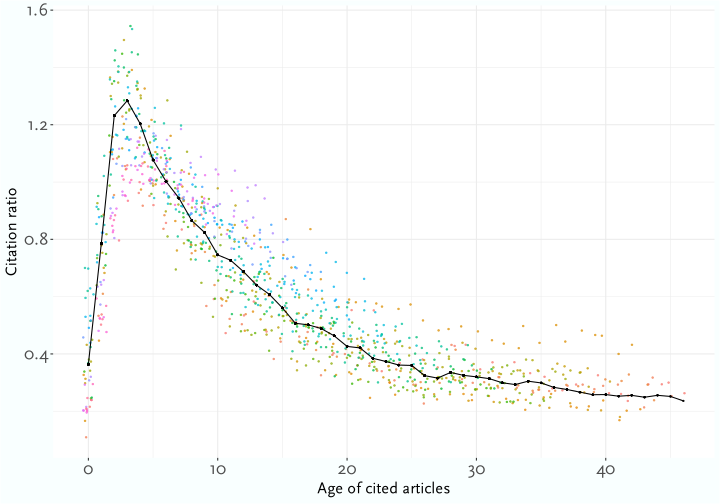
\includegraphics[keepaspectratio]{apc-2025-50_files/figure-pdf/fig-ageeffecteverything-1.pdf}}

}

\caption{\label{fig-ageeffecteverything}Age effects from 1970 onwards on
a single graph, with the overall averrage shown.}

\end{figure}%

The mean curve in Figure~\ref{fig-ageeffecteverything} is really similar
to the unadjusted age curve in Figure~\ref{fig-overall-age}. This is
what I meant earlier by saying that after a lot of calculations, we'd
get back to the same aging curve that we got from the simplest possibe
measure.

The calculations did have one really notable effect though. The
unadjusted age numbers give us a sensible aging curve overall, but they
give us an absurd aging curve for individual years. For most years in
the dataset, the year they are most cited is not two to five years after
initial publication; it is 2021. The point of the various adjustments in
this section has been to make better sense of what's happening in
individual years.

The result is the striking lack of outliers in
Figure~\ref{fig-ageeffecteverything}. All the individual data points are
fairly close to the mean. There is some deviation, and there would be
much more if I included the earlier years where the data is much
noisier. The deviation there is will be the focus of much of the rest of
this paper. Still, it's notable how consistent the age curve is, once we
use citation ratio to account for period effects.

There are two particularly interesting features
Figure~\ref{fig-ageeffecttibble-early} and
Figure~\ref{fig-ageeffecttibble-late} that are a little hard to see in
the big graph. In Figure~\ref{fig-peakratio}, I've graphed the maximum
value the citation ratio reaches for each year of initial publication.
This is a bit misleading before 1965, because I don't have enough data
to calculate citation ratios when the citing year is earlier than that,
so it might have left off what would have been the high point. But from
then on it's useful.

\begin{figure}

\centering{

\pandocbounded{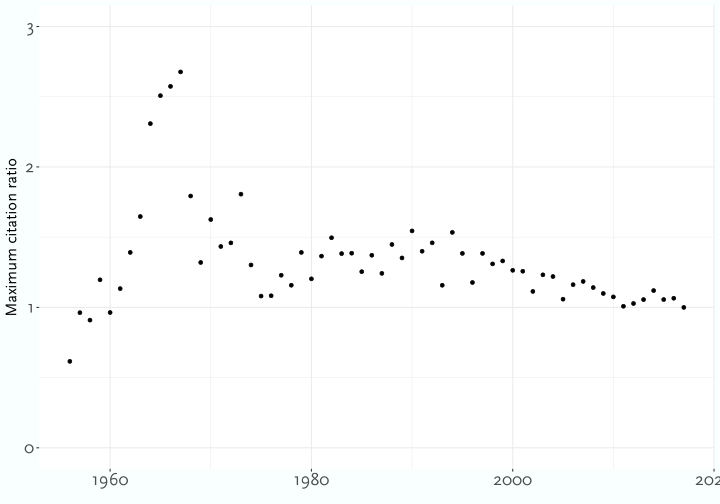
\includegraphics[keepaspectratio]{apc-2025-50_files/figure-pdf/fig-peakratio-1.pdf}}

}

\caption{\label{fig-peakratio}The maximum citation ratio in each facet
in Figure~\ref{fig-ageeffecttibble-early} and
Figure~\ref{fig-ageeffecttibble-late}.}

\end{figure}%

After the initial jump upwards, and the very high numbers in the
mid-1960s, the trend is a decline. In Figure~\ref{fig-peakratiotime}
I've graphed out which age those peaks are hit at, for different years
of initial publication starting in 1963.

\begin{figure}

\centering{

\pandocbounded{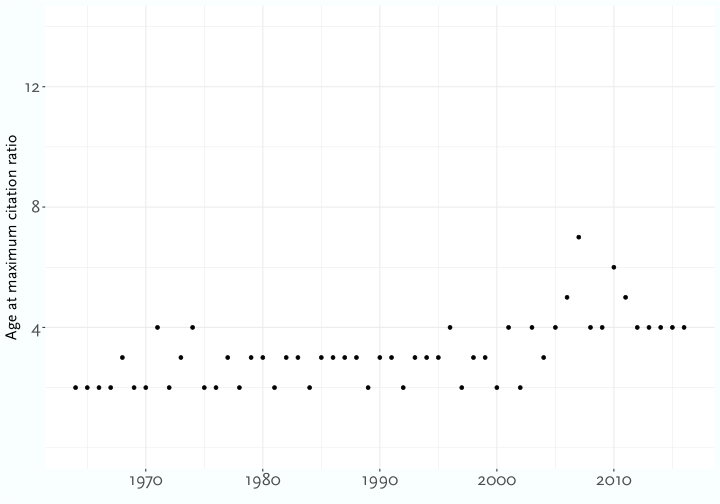
\includegraphics[keepaspectratio]{apc-2025-50_files/figure-pdf/fig-peakratiotime-1.pdf}}

}

\caption{\label{fig-peakratiotime}For each original publication year,
the age it hits maximum citation ratio.}

\end{figure}%

In Figure~\ref{fig-peakratiotime}, the graph is going slightly upwards.
Putting these last two figures together, we get the claim I was
gesturing at earlier: citation curves are getting flatter. The peaks are
coming later, and they are lower.

Finally, I want to note how much variation there is hidden within all
the graphs I've shown so far. I'm mostly here classifying articles
simply by their publication year. If we used more fine-grained
classifications, some of the results would look rather different. In
Figure~\ref{fig-ageeffecteverything-high} and
Figure~\ref{fig-ageeffecteverything-low} I've shown what happens to
Figure~\ref{fig-ageeffecteverything} if we first restrict attention to
articles with 15 or more citations, and then to articles with fewer than
15 citations.\footnote{I picked this threshold because there are
  approximately as many citations to articles with at least that many
  citations as to the other articles.} Obviously in the first graph the
values will be higher; highly cited articles are, indeed, cited more
often. But what I want to highlight here is the different shape of the
curves.

\begin{figure}

\centering{

\pandocbounded{\includegraphics[keepaspectratio]{apc-2025-50_files/figure-pdf/fig-ageeffecteverything-high-1.pdf}}

}

\caption{\label{fig-ageeffecteverything-high}A version of
Figure~\ref{fig-ageeffecteverything} just looking at highly cited
articles}

\end{figure}%

\begin{figure}

\centering{

\pandocbounded{\includegraphics[keepaspectratio]{apc-2025-50_files/figure-pdf/fig-ageeffecteverything-low-1.pdf}}

}

\caption{\label{fig-ageeffecteverything-low}A version of
Figure~\ref{fig-ageeffecteverything} just looking at not so highly cited
articles}

\end{figure}%

Both graphs rise rapidly to a peak two to five years after publication,
and then descend. But from that similarity, the differences are
striking. For the highly cited articles, there is barely any dropoff by
years 8 to 10. For the others, the dropoff starts in earnest in year 4,
and by year 10, the average value is half of the peak. That graph
doesn't quite go to 0, but mostly these articles are not making much
impact after a couple of decades. On the other hand, for the highly
cited articles, the age effects are very gradual. Several decades after
their publication, they are (on average) being cited 2/3 as often as at
their peak (adjusting for period effects).

I think there is an important lesson in this. If the way you think about
citations in philosophy comes from looking the history of famous
articles, you'll get a misleading impression. The citation pattern for a
highly cited article isn't like the citation pattern for a regular
article, just scaled up. It has a very different temporal structure.

None of this a priori. There could be relatively rarely cited articles
that get frequently cited long after their publication. Indeed, there
are such papers in the database. Norman Malcolm's ``Dreaming and
Scepticism'' (\citeproc{ref-WOSA1975KG87100002}{Curley 1975}) didn't get
much attention in the journals when it was firs published, but has been
picked up a bit recently because of an increase in work on dreams. And
there could be articles that are the center of attention for a while
then get fewer citations. Some papers on supervenience fit that
description (e.g., Difrisco (\citeproc{ref-WOS000443474300002}{2018})),
as well as some papers in philosophy of science. But in general, highly
cited articles are highly cited not because they have a flurry of
activity, but because they remain part of the conversation for years
after publication.

\section{Cohort Effects}\label{sec-cohort}

So far we've seen how period effects and age effects between them can
explain a lot of the trends we see in citation patterns. But there are
systematic deviations from those patterns which remain. In
Figure~\ref{fig-fourdeviations}, I've shown some of these. Each graph
shows the citation ratio for articles published in a particular year, as
compared to the average citation ratio at different ages.

\begin{figure}

\begin{minipage}{0.50\linewidth}

\centering{

\pandocbounded{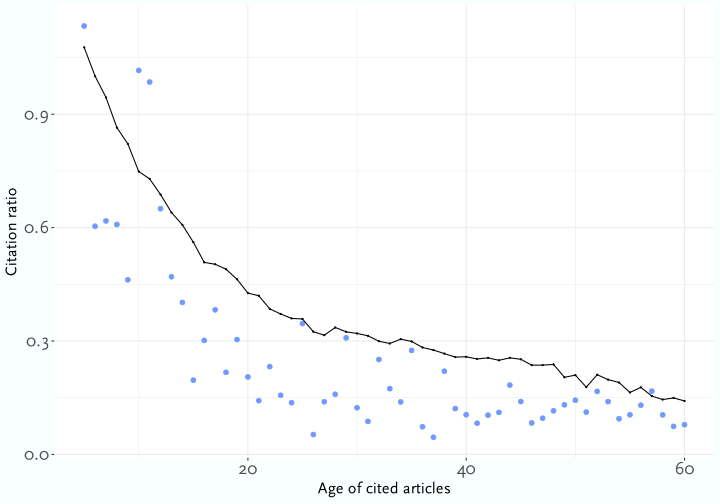
\includegraphics[keepaspectratio]{apc-2025-50_files/figure-pdf/fig-fourdeviations-1.pdf}}

}

\subcaption{\label{fig-fourdeviations-1}1961}

\end{minipage}%
%
\begin{minipage}{0.50\linewidth}

\centering{

\pandocbounded{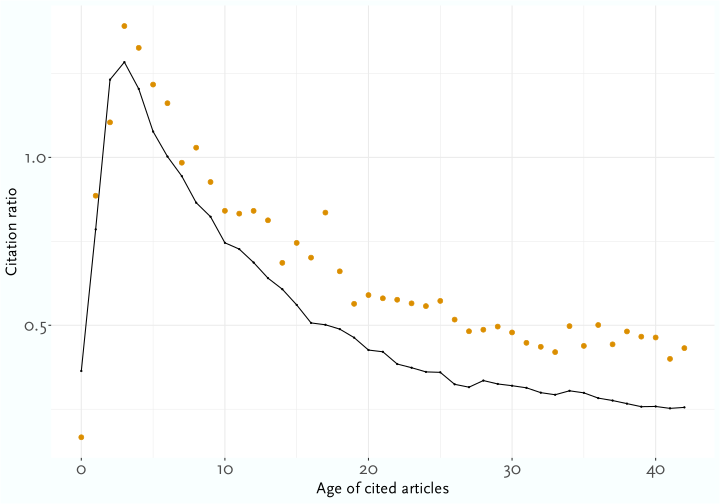
\includegraphics[keepaspectratio]{apc-2025-50_files/figure-pdf/fig-fourdeviations-2.pdf}}

}

\subcaption{\label{fig-fourdeviations-2}1979}

\end{minipage}%
\newline
\begin{minipage}{0.50\linewidth}

\centering{

\pandocbounded{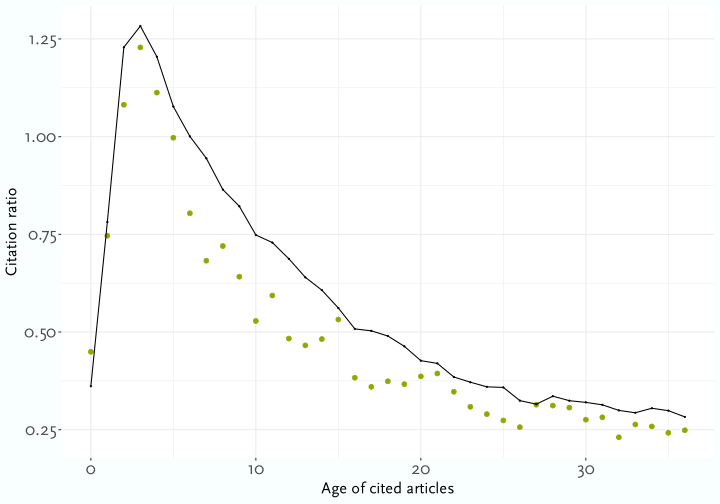
\includegraphics[keepaspectratio]{apc-2025-50_files/figure-pdf/fig-fourdeviations-3.pdf}}

}

\subcaption{\label{fig-fourdeviations-3}1985}

\end{minipage}%
%
\begin{minipage}{0.50\linewidth}

\centering{

\pandocbounded{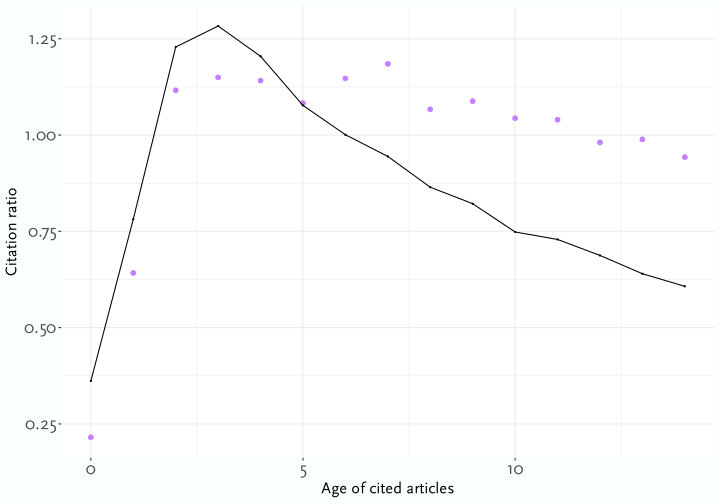
\includegraphics[keepaspectratio]{apc-2025-50_files/figure-pdf/fig-fourdeviations-4.pdf}}

}

\subcaption{\label{fig-fourdeviations-4}2007}

\end{minipage}%

\caption{\label{fig-fourdeviations}Mean annual citations to different
article kinds.}

\end{figure}%

In 1961 and 1985, the yearly values are predominantly below the mean
line. In 1979 and 2007, they are predominantly above it, though this
isn't true for the first few years of the 2007 data. Note that the
graphs have different lengths. Everything stops in 2024. And the 1961
data is cut off a little on the left because we only start calculating
citation ratios in 1965. That's why the line showing the mean is
differently shaped that year.

For each of year of original publication, we can calculate the mean
difference between the citation ratio for that year, and the mean
citation ratio for articles that age. That tells us how often articles
published that year are cited, compared to how often you'd expect them
to be cited knowing just the age and period effects. The results are in
Figure~\ref{fig-cohort}.

\begin{figure}

\centering{

\pandocbounded{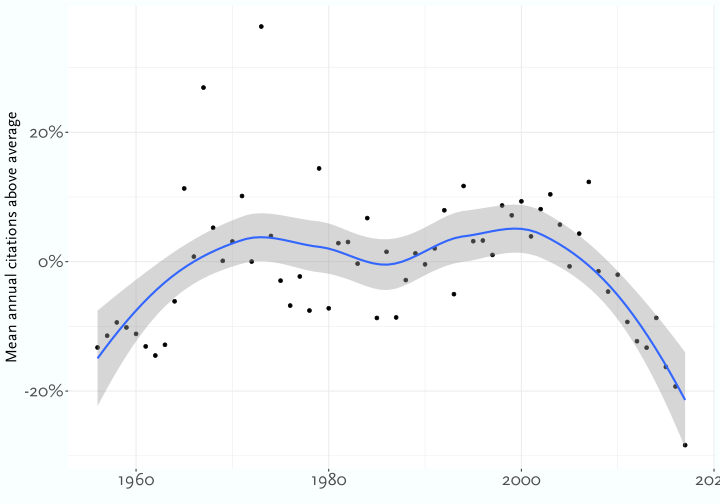
\includegraphics[keepaspectratio]{apc-2025-50_files/figure-pdf/fig-cohort-1.pdf}}

}

\caption{\label{fig-cohort}Cohort effects for different publication
years.}

\end{figure}%

A couple of quick technical notes on Figure~\ref{fig-cohort}. I've added
a smoothed curve over the graph to help make some of the features of it
stand out. And in calculating the mean, I only included years where we
had at least five years worth of data to calculate the mean age effect.
So that means I haven't included what happens to 1955 papers when they
are cited after 2019. There isn't nearly enough data to say what one
would `expect' the usual aging curve to be at those points.

On the face of it, there are five periods in the graph.

\begin{enumerate}
\def\labelenumi{\arabic{enumi}.}
\tightlist
\item
  Journal articles published before the mid-1960s are very rarely cited.
\item
  After that, and especially in the early 1970s, a flurry of very highly
  cited articles are published.
\item
  Then there is a period of stagnation, where things mostly don't return
  to the lows of per-1965, but are consistently below 0.
\item
  There is an uptick starting in the mid-1990s, and peaking dramatically
  in 2007.
\item
  Then there is a rather dramatic drop off, almost immediately after the
  high of 2007.
\end{enumerate}

The first couple of trends make sense; the latter three less so. The
rest of this paper (before the methodology section) will be about
explaining what's going on here, and seeing what it can tell us both
about the history of philosophy, and the history of the philosophy
profession.

Before 1965, the philosophical work with the most lasting significance
was not done in journals. And those works of lasting significance that
were in things one might call journals often are not indexed by Web of
Science. So we don't have ``Is Knowledge Justified True Belief?''
(\citeproc{ref-Gettier1963}{Gettier 1963}) because they don't index
\emph{Analysis} until 1975, and we don't have Austin's two most
important papers - ``Ifs and Cans'' and ``A Plea for Excuses''
(\citeproc{ref-Austin1956}{Austin 1956a},
\citeproc{ref-Austin1956b}{1956b}) because their venues aren't indexed
as journals at all. We do have important papers by Frege
(\citeproc{ref-WOSA1956CHJ4400001}{1956}), W. van O. Quine
(\citeproc{ref-WOSA1956CEQ2500001}{1956}), Grice
(\citeproc{ref-WOSA1957CGZ6000005}{1957}), Anscombe
(\citeproc{ref-WOSA1958CDL1000001}{1958}), Smart
(\citeproc{ref-WOSA1959CGZ6600001}{1959}), and Davidson
(\citeproc{ref-WOSA1963CEU0700001}{1963}). But these made much less
impact than books from the same time, especially \emph{Intention}
(\citeproc{ref-Anscombe1957}{Anscombe 1957}), \emph{Word and Object}
(\citeproc{ref-Quine1960}{W. V. O. Quine 1960}) and \emph{The Structure
of Scientific Revolutions} (\citeproc{ref-Kuhn1962}{Kuhn 1962}).

Then starting in the late 1960s, almost every area of philosophy got
turned upside down, with much of the action happening in journals. The
two most important works of the period, \emph{A Theory of Justice}
(\citeproc{ref-Rawls1971}{Rawls 1971}) and \emph{Naming and Necessity}
(\citeproc{ref-Kripke1980}{Kripke {[}1972{]} 1980}), were not in
journals. But articles in journals did make revolutionary changes in
many fields, including:

\begin{itemize}
\tightlist
\item
  Free will (\citeproc{ref-WOSA1969Y444700002}{Frankfurt 1969a},
  \citeproc{ref-10.2307_2024717}{1971});
\item
  Practical ethics (\citeproc{ref-WOSA1971Y116900003}{Thomson 1971};
  \citeproc{ref-WOSA1972Z066400001}{Singer 1972});
\item
  Meaning and reference (\citeproc{ref-10.2307_2025079}{Putnam 1973});
\item
  Philosophy of mathematics (\citeproc{ref-10.2307_2025075}{Benacerraf
  1973});
\item
  Causation (\citeproc{ref-10.2307_2025310}{Lewis 1973};
  \citeproc{ref-10.2307_2025096}{Kim 1973}); and
\item
  Personal identity (\citeproc{ref-WOSA1971Y036400001}{Parfit 1971})
\end{itemize}

As well there were a surprising number of papers that weren't as
influential straight away, but came to play a big role the later
literature. This group includes papers by Fred Dretske
(\citeproc{ref-WOSA1970ZE33800001}{1970}), David Lewis
(\citeproc{ref-WOSA1970ZE32700001}{1970}), Kendall Walton
(\citeproc{ref-WOSA1970Y384700002}{1970}) and Larry Wright
(\citeproc{ref-WOSA1973P242100001}{1973}). That's all to say that the
story that Figure~\ref{fig-cohort} tells about the early 1970s is
plausible. There had never before been a period when there was such a
quantity of high quality work being done in philosophy journals.

To see what is happening after that time, though, we need to look a
little more closely at the data. Figure~\ref{fig-cohort-short} is a
version of Figure~\ref{fig-cohort} just focussing on the first seven
years after publication. That is, for each publication year, it measures
citations of articles published that year in the seven years after they
were published, adjusted in the same way for age and period effects.

\begin{figure}

\centering{

\pandocbounded{\includegraphics[keepaspectratio]{apc-2025-50_files/figure-pdf/fig-cohort-short-1.pdf}}

}

\caption{\label{fig-cohort-short}A version of Figure~\ref{fig-cohort}
restricted to citations from the first seven years after publication.}

\end{figure}%

Figure~\ref{fig-cohort-short} is measuring how often articles from a
year are cited, soon after publication, compared to articles cited
before them and, to a lesser extent, immediately after them. So the high
numbers in the early 1960s are not showing that articles from that time
were highly cited in an absolute sense, just that they were cited much
more than articles from the 1950s were.

After that boom, and the one-off year of 1973, things are reasonably
steady through the mid-2000s. Then, especially after 2007, there is a
massive drop. Why is that happening? Part of the answer is shown in
Figure~\ref{fig-cohort-long}, which is the same measure but only for
citations after the first seven years.

\begin{figure}

\centering{

\pandocbounded{\includegraphics[keepaspectratio]{apc-2025-50_files/figure-pdf/fig-cohort-long-1.pdf}}

}

\caption{\label{fig-cohort-long}A version of Figure~\ref{fig-cohort}
restricted to citations from after the first seven years after
publication.}

\end{figure}%

The differences between Figure~\ref{fig-cohort-short} and
Figure~\ref{fig-cohort-long} are striking. After both graphs go up in
the early 1970s, and down in the early 1980s, they are strongly
anti-correlated. Between the mid-1980s and mid-1990s, short term
citations are up, and long term citations are down. After around 1995,
short term citations start cratering, and long term citations are as
high as ever?

What could explain this pattern? In the next three sections, going to
suggest three overlapping accounts: one involving technology, one
involving content, and one involving culture.

\section{Technology and Citations}\label{sec-technology}

As I noted at the top, I feel a common view is that the primary role of
electronic publication has been to speed up \emph{distribution}. This
view is not borne out by the data. If that were the case, you'd expect
to see short term, especially very short term, citations rising over
time.

Printing and postage was a pretty mature technology by the late
twentieth century. We weren't waiting for steam ships to bring the
latest issues of journals to distant shores. The technology used for
distributing philosophy journals was the same technology used for
distributing journals in medicine and other fields where time was of the
essence. From that perspective, the internet would only speed things up
by weeks, maybe months, and this wouldn't really show on a graph in
years.

What is perhaps more surprising is that the prevalence of Online First,
Early View, and other forms of quasi-publication haven't made more of a
difference. They do show up in the data. Until recently, there were zero
articles cited in an earlier year than their official publication year.
If they were cited in manuscript form, as, e.g., ``Demonstratives''
(\citeproc{ref-Kaplan1989}{Kaplan 1989}) often was, these citations
didn't show up in indicies like the one I'm using. Articles cited in
Early View do show up, so we start to see negative citation ages in the
data. But we don't see enough of them to make much of a difference.

The biggest effect of technology was not on distribution but on
\emph{search}. Before the widespread use of computers, there was a much
better system for searching books than for searching journal articles.
Classification systems meant books typically lived on shelves near other
books on the same topic. Card catalogues would list subject matters for
books. Even the title of the book could help track down what it was
about. Finding a journal article on a relevant topic was much harder.
And, it seems, it mostly wasn't done.

My impression is that there was also a notable physical difference
between the ways books and journals were stored and accessed. Almost
every academic has a bookshelf; not as many have large collections of
journals. Occasionally a department would have physical journals on
hand, but often the best way to access journals was to walk across
campus to a library. On the other hand, accessing a book might involve
walking four steps to a shelf. This physical difference probably
contributed to the relative prominence of books and articles in
bibliographies.

There often was an exception to this general claim about access. (At
least, this was true in any pre-twentieth century department I was
familiar with, but I think it was moderately widespread.) Departments
would sometimes keep the latest issues of journals in a department
library or common room. Those would be much more prominent, and easy to
access. I'm not sure whether this explains why so many of the journal
citations pre-1995 are to very recent journals, but it probably helped.

So that I think is part of the story. Before the widespread adoption of
computers, old journal articles were very hard to find. This changed a
little with the advent of electronic, and hence easily searchable,
versions of \emph{Philosophers' Index}, and changed a lot when journals
went online. And that's part of why older articles, and especially older
articles that are not classics, are now more widely cited.

\section{Content Changes}\label{sec-content}

Another part of the story is that the centre of gravity of philosophy
publishing changes over the time period we're looking at. And it does so
in a way that turns out to matter for which kinds of articles are cited.

Through at least the early 2000s, analytic philosophy is in what Sider
(\citeproc{ref-Sider2020}{2020, 2}) calls the ``modal era''. One aspect
of this era, one that Sider particularly highlights, is that questions
about essence were equated with questions about necessity in a way that
they weren't either before or after the era.\footnote{It was usual,
  during this era, to take the necessity of origins thesis and the
  origin essentialism thesis to not just be mutually supporting, but to
  be literally identical. I don't think that identity claim would be
  widely endorsed either before 1970 or after 2010.} This should be
taken as a symptom of the era, not the definition of it. What's really
defining of the era was the way modality became central to disputes
across the discipline.

Consider, for example, what Frank Jackson
(\citeproc{ref-Jackson1998}{1998}) called the `location problem', i.e.,
the problem of how to locate in the world something that the philosopher
thinks exists, and is not fundamental. Jackson argues that saying how to
locate the non-fundamental in the fundamental is a compulsory question
for anyone doing `serious metaphysics', and the one and only answer to
it will involve modality. As he says,

\begin{quote}
When does a putative feature of our world have a place in the account
some serious metaphysics tells of what our world is like? I have already
mentioned one answer: if the feature is entailed by the account told in
the terms favoured by the metaphysics in question, it has a place in the
account told in the favoured terms. This is hardly controversial
considered as a sufficient condition, but, I will now argue, it is also
a necessary condition: the one and only way of having a place in an
account told in some set of preferred terms is by being entailed by that
account---a view I will refer to as the entry by entailment thesis.
(\citeproc{ref-Jackson1998}{Jackson 1998, 5})
\end{quote}

Now Jackson went on to say other things about entailment that were not
widely endorsed. But at this early stage in the book, I think he was
largely expressing conventional wisdom.\footnote{The only thing really
  puzzling about this passage is the claim about the relative
  controversialness of the necessity and sufficiency entailment as a
  solution to the location problem. After all, Horgan
  (\citeproc{ref-WOSA1982NN35300003}{1982}) had already raised problems
  for it. So too had Fine (\citeproc{ref-Fine1994b}{1994}), in a way
  that would become very important a few years later, but that was not
  playing a major role in the literature, especially when Jackson
  delivered the Locke lectures this book was based on.} In a review that
disagrees with many parts of the book, Stephen Yablo
(\citeproc{ref-Yablo2000Jackson}{2000, 20}) says ``Not many eyebrows
will be raised by Jackson's view that metaphysics is committed to `entry
by entailment' theses.'' That is, the quoted parts are not
controversial, especially the one that Jackson flags as being ever so
slightly more controversial.

The idea that entailment, i.e., necessitation, had been central to
understanding how the non-fundamental relates to the fundamental had
been central to philosophy for many years by this point. (To be clear,
Jackson isn't claiming great novelty at this point of his book; the big
claim he's building towards is that the necessitation is a priori
knowable.) We can see just how central it is by using a slightly
different statistic to what I've used so far: grand-citations.

Say that the number of grand-citations an article \emph{a} has is the
number of triples ⟨\emph{a}, \emph{b}, \emph{c}⟩ such that \emph{c}
cites \emph{b} and \emph{b} cites \emph{a}. It's the sum of the number
of citations of articles that cite \emph{a}. If we look at
grand-citations over time, they show David Lewis's centrality to the
philosophy journals. Through 2021, six of the eight articles with the
most grand-citations are by Lewis. If instead we look at particular
times, we see the changing face of the journals. Grand-citations take
some time to accrue, so I'll look at twenty year periods. In particular,
for various years, I'll look at which articles published in the
preceeding twenty years had the most grand-citations through that year.

Table~\ref{tbl-grand-cite-2000} lists which articles, published from
1980 onwards, had the most grand-citations through 2000.


\begin{longtable}[]{@{}
  >{\raggedleft\arraybackslash}p{(\linewidth - 6\tabcolsep) * \real{0.0388}}
  >{\raggedright\arraybackslash}p{(\linewidth - 6\tabcolsep) * \real{0.7597}}
  >{\raggedleft\arraybackslash}p{(\linewidth - 6\tabcolsep) * \real{0.0775}}
  >{\raggedleft\arraybackslash}p{(\linewidth - 6\tabcolsep) * \real{0.1240}}@{}}

\caption{\label{tbl-grand-cite-2000}The 10 articles from the 1980s and
1990s with the most grand-citations through 2000.}

\tabularnewline

\toprule\noalign{}
\begin{minipage}[b]{\linewidth}\raggedleft
Rank
\end{minipage} & \begin{minipage}[b]{\linewidth}\raggedright
Article
\end{minipage} & \begin{minipage}[b]{\linewidth}\raggedleft
Citations
\end{minipage} & \begin{minipage}[b]{\linewidth}\raggedleft
Grand-Citations
\end{minipage} \\
\midrule\noalign{}
\endhead
\bottomrule\noalign{}
\endlastfoot
1 & Terrence Horgan
(\citeproc{ref-WOSA1982NN35300003}{1982})
``Supervenience and Microphysics'' & 36 & 318 \\
2 & Tyler Burge
(\citeproc{ref-WOSA1986AYX3200001}{1986})
``Individualism and Psychology'' & 82 & 316 \\
3 & David Lewis
(\citeproc{ref-WOSA1983RR51600001}{1983})
``New Work for a Theory of Universals'' & 86 & 308 \\
4 & Paul M. Churchland
(\citeproc{ref-WOSA1981LD54600001}{1981})
``Eliminative Materialism and the Propositional Attitudes'' & 94 &
299 \\
5 & John Haugeland
(\citeproc{ref-WOSA1982NC42600008}{1982})
``Weak Supervenience'' & 40 & 258 \\
6 & Jaegwon Kim
(\citeproc{ref-WOSA1982NC90700004}{1982})
``Psychophysical Supervenience'' & 40 & 245 \\
7 & Ruth Garrett Millikan
(\citeproc{ref-WOSA1989AA09400006}{1989})
``In Defense of Proper Functions'' & 43 & 232 \\
8 & Jon Barwise and Robin Cooper
(\citeproc{ref-WOSA1981LH67300001}{1981})
``Generalized Quantifiers and Natural-Language'' & 83 & 221 \\
9 & John Bigelow and Robert Pargetter
(\citeproc{ref-WOSA1987G947600001}{1987})
``Functions'' & 30 & 220 \\
10 & Jaegwon Kim
(\citeproc{ref-WOSA1984TV24600001}{1984})
``Concepts of Supervenience'' & 87 & 219 \\

\end{longtable}

I've included the names of the articles on this table to make vivid how
central supervenience was to the literature at this time.\footnote{The
  story of the relationship between twentieth century work on functions
  and twenty-first century work on mechanisms is interesting, but for
  another time.} Four of the articles here have the word `supervenience'
in the title! At the center of this literature stood Jaegwon Kim. The
citation data I have somewhat \emph{underestimates} his influence,
because people often cited his edited collection \emph{Supervenience and
Mind} (\citeproc{ref-Kim1993}{\emph{Supervenience and Mind} 1993}), and
those citations are usually not tracked by Web of Science.\footnote{I
  had originally planned to include much more on how individual papers
  rise and fall in the citation indices, but this turned out to be less
  interesting than I thought. Most of the biggest `falls' are just when
  a paper stops being cited because a book gets cited. Sometimes what
  gets cited is the reprint of the paper itself, as happened here.
  Sometimes the book supersedes the article. So you see a drop in
  citations to Rawls's article ``Justice as Fairness: Political not
  Metaphysical'' (\citeproc{ref-WOSA1985APA8500001}{Rawls 1985}) after
  his book \emph{Justice as Fairness: A Restatement}
  (\citeproc{ref-Rawls2001}{Rawls 2001}) came out. Looking at
  grand-citations somewhat mitigates these issues, since they still
  track how much the articles that originally cited the older article
  are being picked up.}

When we move into the 2000s, the focus shifts dramatically, as we see in
Table~\ref{tbl-grand-cite-2010}.


\begin{longtable}[]{@{}
  >{\raggedleft\arraybackslash}p{(\linewidth - 6\tabcolsep) * \real{0.0347}}
  >{\raggedright\arraybackslash}p{(\linewidth - 6\tabcolsep) * \real{0.7847}}
  >{\raggedleft\arraybackslash}p{(\linewidth - 6\tabcolsep) * \real{0.0694}}
  >{\raggedleft\arraybackslash}p{(\linewidth - 6\tabcolsep) * \real{0.1111}}@{}}

\caption{\label{tbl-grand-cite-2010}The 10 articles from the 1990s and
2000s with the most grand-citations through 2010.}

\tabularnewline

\toprule\noalign{}
\begin{minipage}[b]{\linewidth}\raggedleft
Rank
\end{minipage} & \begin{minipage}[b]{\linewidth}\raggedright
Article
\end{minipage} & \begin{minipage}[b]{\linewidth}\raggedleft
Citations
\end{minipage} & \begin{minipage}[b]{\linewidth}\raggedleft
Grand-Citations
\end{minipage} \\
\midrule\noalign{}
\endhead
\bottomrule\noalign{}
\endlastfoot
1 & David Lewis
(\citeproc{ref-WOSA1996VY21200001}{1996})
``Elusive Knowledge'' & 182 & 665 \\
2 & Keith DeRose
(\citeproc{ref-WOSA1995RC31600001}{1995})
``Solving the Skeptical Problem'' & 145 & 604 \\
3 & Stephen Yablo
(\citeproc{ref-WOSA1992JA62400001}{1992})
``Mental Causation'' & 126 & 572 \\
4 & Keith DeRose
(\citeproc{ref-WOSA1991GL32100002}{1991})
``Epistemic Possibilities'' & 40 & 519 \\
5 & Tyler Burge
(\citeproc{ref-WOSA1993ML38000001}{1993})
``Content Preservation'' & 136 & 502 \\
6 & Karen Neander
(\citeproc{ref-WOSA1991FQ15000002}{1991})
``Functions as Selected Effects: The Conceptual Analyst's Defense'' & 89
& 480 \\
7 & Keith DeRose
(\citeproc{ref-WOSA1992KB29500008}{1992})
``Contextualism and Knowledge Attributions'' & 79 & 430 \\
8 & Mark Johnston
(\citeproc{ref-WOSA1992KC39800002}{1992})
``How To Speak of the Colors'' & 93 & 423 \\
9 & C. B. Martin
(\citeproc{ref-WOSA1994MT56900001}{1994})
``Dispositions and Conditionals'' & 82 & 401 \\
10 & Michael B. Burke
(\citeproc{ref-WOSA1992HC13100003}{1992})
``Copper Statues and Pieces of Copper: A Challenge To the Standard
Account'' & 45 & 395 \\

\end{longtable}

Even more than with the Table~\ref{tbl-grand-cite-2000}, one
complication with Table~\ref{tbl-grand-cite-2010} is that I'm using a
counting statistic, so it is biased in favor of older papers with more
time to accrue citations. That said, the top takeaway is fairly clear.
The biggest single topic over this time was contextualism in
epistemology, with the big papers by Lewis
(\citeproc{ref-WOSA1996VY21200001}{1996}) and DeRose
(\citeproc{ref-WOSA1995RC31600001}{1995}) at the center of things. What
I want to focus particularly on, though, is another DeRose paper on that
list: ``Epistemic Possibilities''. It has fewer cites than any other
paper there, but the fourth most grand-cites. The way this came about is
revealing of changes in the discipline, and particularly in citation
practices.

DeRose's paper is an important early contribution to debates about
epistemic modals that became very active in the 2000s. This activity was
partially due to the intrinsic interest of the subject. But it was also
due to the way that epistemic modals sit at the intersection of three
enormous debates that were going on at the time. One was epistemic
contextualism, which you can see the impact of in
Table~\ref{tbl-grand-cite-2010}. The second was about the nature of
context-sensitivity in language, with work by Stanley and Szabó
(\citeproc{ref-WOS000088616400001}{2000}) at the center of
it.\footnote{I won't include the full table, but if you created a table
  like Table~\ref{tbl-grand-cite-2010} for the twenty years through
  2015, Stanley and Szabó's paper would be on it.} And the third was
about the possibility of a modern form of relativism, with the central
figure here being John MacFarlane (\citeproc{ref-MacFarlane2014}{2014}).
Papers on epistemic modals were influenced by, and in turn influenced,
all three of these debates.\footnote{For particularly notable examples,
  see the papers by Andy Stanley and Szabó
  (\citeproc{ref-WOS000088616400001}{2000}), Seth Yalcin
  (\citeproc{ref-WOS000251545300007}{2007}), and Tamina Stephenson
  (\citeproc{ref-WOS000255667800003}{2007}).}

These debates had an impact on how citations worked in philosophy in a
few ways. One was in virtue of the fact that they were largely new
topics, there wasn't an established canon that writers could assume
familiarity with. So they needed to cite more papers to establish the
debate. It wasn't necessary to cite Putnam
(\citeproc{ref-10.2307_2025079}{1973}) or Kripke
(\citeproc{ref-Kripke1980}{{[}1972{]} 1980}) every time you wanted to
distinguish necessity from a priority; the reader in the 1990s could be
assumed to know where the distinction came from. But the reader in the
2000s could not be assumed to know about work by Fred Dretske
(\citeproc{ref-WOSA1970ZE33800001}{1970}), G. C. Stine
(\citeproc{ref-WOSA1976EK38300003}{1976}), or Stewart Cohen
(\citeproc{ref-WOSA1987K730800002}{1987}).

Perhaps more significant was that these debates, especially the second
and third, were much more interdisciplinary than debates about modality
had been. Many of the writers were primarily in linguistics, not
philosophy, and the philosophers were reading more linguistics than ever
before. The citation norms in linguistics, like in most other social
sciences, required more citations than the norms in philosophy did. They
didn't require more citation than the philosophy norms in the 2020s, but
much more than philosophy in the 1990s. So these debates, which became
important across a range of journals from the mid 2000s onwards, tended
to have many more citations than before.

To back up the claims in the last two paragraphs I need one more
statistic. (The last one I'll introduce in this essay!) This is a way of
adjusting for age, period, and cohort effects all at once.\footnote{I
  haven't used it above because using it doesn't help much in separating
  out the three effects.} For an article \emph{a} published in year
\emph{y}, say that the \textbf{weight} of its citations in year \emph{z}
is the number of times it is cited in \emph{z}, divided by the average
number of citations that articles in year \emph{y} get in \emph{z}. So
it's just the measure of how often the article is cited, compared to how
often you'd expect it to be cited knowing just the publication year and
citation year. We'll be interested in three statistics. The
\textbf{overall weight} of an article is the average of its weight over
each year between the year after its publication and 2024. The
\textbf{short-term weight} is the average of its weight over the seven
years after it was published. And the \textbf{long-term weight} is the
average of its weight from eight years after publication to 2024. For
individual articles, this measure is too noisy to be particularly
meaningful. If we take the averages of all articles published in a year,
the average weight at any time is, by definition, 1. So that's not much
help either. But for medium sized classes of articles, the average
weights can be interesting. In particular, looking at the average
weights of articles which cite some particular prominent article are
interesting.

This is a variant on grand-citations, and like grand-citations, it takes
some time to


\begin{longtable}[]{@{}
  >{\raggedleft\arraybackslash}p{(\linewidth - 6\tabcolsep) * \real{0.0382}}
  >{\raggedright\arraybackslash}p{(\linewidth - 6\tabcolsep) * \real{0.7634}}
  >{\raggedleft\arraybackslash}p{(\linewidth - 6\tabcolsep) * \real{0.0763}}
  >{\raggedleft\arraybackslash}p{(\linewidth - 6\tabcolsep) * \real{0.1221}}@{}}

\caption{\label{tbl-grand-cite-2020}The 10 articles from the 1990s and
2000s with the most grand-citations through 2020.}

\tabularnewline

\toprule\noalign{}
\begin{minipage}[b]{\linewidth}\raggedleft
Rank
\end{minipage} & \begin{minipage}[b]{\linewidth}\raggedright
Article
\end{minipage} & \begin{minipage}[b]{\linewidth}\raggedleft
Citations
\end{minipage} & \begin{minipage}[b]{\linewidth}\raggedleft
Grand-Citations
\end{minipage} \\
\midrule\noalign{}
\endhead
\bottomrule\noalign{}
\endlastfoot
1 & Peter Machamer, Lindley Darden, and Carl F. Craver
(\citeproc{ref-WOS000087305900001}{2000})
``Thinking About Mechanisms'' & 402 & 2807 \\
2 & James Pryor
(\citeproc{ref-WOS000165361800002}{2000})
``The Skeptic and the Dogmatist'' & 288 & 1680 \\
3 & David Lewis
(\citeproc{ref-WOS000089124200002}{2000})
``Causation as Influence'' & 173 & 1647 \\
4 & Jeremy Fantl and Matthew McGrath
(\citeproc{ref-WOS000181094500003}{2002})
``Evidence, Pragmatics, and Justification'' & 149 & 1557 \\
5 & Jonathan Schaffer
(\citeproc{ref-WOS000272855000002}{2010})
``Monism: The Priority of the Whole'' & 215 & 1429 \\
6 & Jason Stanley and Timothy Williamson
(\citeproc{ref-WOS000170277300002}{2001})
``Knowing How'' & 208 & 1418 \\
7 & Keith DeRose
(\citeproc{ref-WOS000184740400001}{2003})
``Assertion, Knowledge, and Context'' & 170 & 1415 \\
8 & David Christensen
(\citeproc{ref-WOS000207419300002}{2007})
``Epistemology of Disagreement: The Good News'' & 206 & 1387 \\
9 & Nishi Shah
(\citeproc{ref-WOS000224335200001}{2003})
``How Truth Governs Belief'' & 135 & 1303 \\
10 & Adam Elga
(\citeproc{ref-WOS000249103800005}{2007b})
``Reflection and Disagreement'' & 216 & 1301 \\

\end{longtable}

\section{Methodology}\label{sec-methodology}

\phantomsection\label{refs}
\begin{CSLReferences}{1}{0}
\bibitem[\citeproctext]{ref-WOSA1956CHJ4200001}
Anscombe, G. E. M. 1956. {``Aristotle and the Sea Battle.''} \emph{Mind}
65 (257): 1--15. \url{https://doi.org/10.1093/mind/65.1.1}.

\bibitem[\citeproctext]{ref-Anscombe1957}
---------. 1957. \emph{Intention}. Oxford: Basil Blackwell.

\bibitem[\citeproctext]{ref-WOSA1958CDL1000001}
---------. 1958. {``Modern Moral Philosophy.''} \emph{Philosophy} 33
(124): 1--19. \url{https://doi.org/10.1017/S0031819100037943}.

\bibitem[\citeproctext]{ref-Austin1956}
Austin, J. L. 1956a. {``A Plea for Excuses.''} \emph{Proceedings of the
Aristotelian Society} 57 (1): 1--30.
\url{https://doi.org/10.1093/aristotelian/57.1.1}.

\bibitem[\citeproctext]{ref-Austin1956b}
---------. 1956b. {``Ifs and Cans.''} \emph{Proceedings of the British
Academy} 42: 109--32.

\bibitem[\citeproctext]{ref-WOSA1981LH67300001}
Barwise, Jon, and Robin Cooper. 1981. {``Generalized Quantifiers and
Natural-Language.''} \emph{Linguistics and Philosophy} 4 (2): 159--219.
\url{https://doi.org/10.1007/BF00350139}.

\bibitem[\citeproctext]{ref-10.2307_2025075}
Benacerraf, Paul. 1973. {``Mathematical Truth.''} \emph{Journal of
Philosophy} 70 (19): 661--79.

\bibitem[\citeproctext]{ref-WOSA1987G947600001}
Bigelow, John, and Robert Pargetter. 1987. {``Functions.''}
\emph{Journal of Philosophy} 84 (4): 181--96.
\url{https://doi.org/10.2307/2027157}.

\bibitem[\citeproctext]{ref-Bump2023}
Bump, Philip. 2023. \emph{The Aftermath: The Last Days of the Baby Boom
and the Future of Power in America}. New York: Penguin Random House.

\bibitem[\citeproctext]{ref-WOSA1986AYX3200001}
Burge, Tyler. 1986. {``Individualism and Psychology.''}
\emph{Philosophical Review} 95 (1): 3--45.
\url{https://doi.org/10.2307/2185131}.

\bibitem[\citeproctext]{ref-WOSA1993ML38000001}
---------. 1993. {``Content Preservation.''} \emph{Philosophical Review}
102 (4): 457--88. \url{https://doi.org/10.2307/2185680}.

\bibitem[\citeproctext]{ref-WOSA1992HC13100003}
Burke, Michael B. 1992. {``Copper Statues and Pieces of Copper: A
Challenge To the Standard Account.''} \emph{Analysis} 52 (1): 12--17.
\url{https://doi.org/10.2307/3328875}.

\bibitem[\citeproctext]{ref-WOS000207419300002}
Christensen, David. 2007. {``Epistemology of Disagreement: The Good
News.''} \emph{Philosophical Review} 116 (2): 187--217.
\url{https://doi.org/10.1215/00318108-2006-035}.

\bibitem[\citeproctext]{ref-WOSA1981LD54600001}
Churchland, Paul M. 1981. {``Eliminative Materialism and the
Propositional Attitudes.''} \emph{Journal of Philosophy} 78 (2): 67--90.
\url{https://doi.org/10.2307/2025900}.

\bibitem[\citeproctext]{ref-WOS000073222300002}
Clark, Andy, and David J. Chalmers. 1998. {``The Extended Mind.''}
\emph{Analysis} 58 (1): 7--19.
\url{https://doi.org/10.1111/1467-8284.00096}.

\bibitem[\citeproctext]{ref-WOSA1987K730800002}
Cohen, Stewart. 1987. {``Knowledge, Context, and Social Standards.''}
\emph{Synthese} 73 (1): 3--26. \url{https://doi.org/10.1007/BF00485440}.

\bibitem[\citeproctext]{ref-WOSA1975BF60100001}
Cummins, Robert. 1975. {``Functional Analysis.''} \emph{Journal of
Philosophy} 72 (20): 741--65. \url{https://doi.org/10.2307/2024640}.

\bibitem[\citeproctext]{ref-WOSA1975KG87100002}
Curley, EM. 1975. {``Dreaming and Conceptual Revision.''}
\emph{Australasian Journal of Philosophy} 53 (2): 119--41.
\url{https://doi.org/10.1080/00048407512341131}.

\bibitem[\citeproctext]{ref-WOSA1963CEU0700001}
Davidson, Donald. 1963. {``Actions, Reasons, and Causes.''}
\emph{Journal of Philosophy} 60 (23): 685--700.
\url{https://doi.org/10.2307/2023177}.

\bibitem[\citeproctext]{ref-WOSA1991GL32100002}
DeRose, Keith. 1991. {``Epistemic Possibilities.''} \emph{Philosophical
Review} 100 (4): 581--605. \url{https://doi.org/10.2307/2185175}.

\bibitem[\citeproctext]{ref-WOSA1992KB29500008}
---------. 1992. {``Contextualism and Knowledge Attributions.''}
\emph{Philosophy and Phenomenological Research} 52 (4): 913--29.
\url{https://doi.org/10.2307/2107917}.

\bibitem[\citeproctext]{ref-WOSA1995RC31600001}
---------. 1995. {``Solving the Skeptical Problem.''}
\emph{Philosophical Review} 104 (1): 1--52.
\url{https://doi.org/10.2307/2186011}.

\bibitem[\citeproctext]{ref-WOS000184740400001}
---------. 2003. {``Assertion, Knowledge, and Context.''}
\emph{Philosophical Review} 111 (2): 167--203.

\bibitem[\citeproctext]{ref-WOS000443474300002}
Difrisco, James. 2018. {``Token Physicalism and Functional
Individuation.''} \emph{European Journal for Philosophy of Science} 8
(3): 309--29. \url{https://doi.org/10.1007/s13194-017-0188-y}.

\bibitem[\citeproctext]{ref-WOSA1970ZE33800001}
Dretske, Fred. 1970. {``Epistemic Operators.''} \emph{Journal of
Philosophy} 67 (24): 1007--23. \url{https://doi.org/10.2307/2024710}.

\bibitem[\citeproctext]{ref-Elga2007}
Elga, Adam. 2007a. {``Reflection and Disagreement.''} \emph{No{û}s} 41
(3): 478--502. \url{https://doi.org/10.1111/j.1468-0068.2007.00656.x}.

\bibitem[\citeproctext]{ref-WOS000249103800005}
---------. 2007b. {``Reflection and Disagreement.''} \emph{Noûs} 41 (3):
478--502. \url{https://doi.org/10.1111/j.1468-0068.2007.00656.x}.

\bibitem[\citeproctext]{ref-WOS000181094500003}
Fantl, Jeremy, and Matthew McGrath. 2002. {``Evidence, Pragmatics, and
Justification.''} \emph{Philosophical Review} 111 (1): 67--94.
\url{https://doi.org/10.1215/00318108-111-1-67}.

\bibitem[\citeproctext]{ref-Fine1994b}
Fine, Kit. 1994. {``Essence and Modality.''} \emph{Philosophical
Perspectives} 8: 1--16. \url{https://doi.org/10.2307/2214160}.

\bibitem[\citeproctext]{ref-WOSA1984SS95000001}
Fraassen, Bas C. van. 1984. {``Belief and the Will.''} \emph{Journal of
Philosophy} 81 (5): 235--56.

\bibitem[\citeproctext]{ref-Frankfurt1969}
Frankfurt, Harry G. 1969b. {``Alternate Possibilities and Moral
Responsibility.''} \emph{Journal Of Philosophy} 66 (23): 829--39.
\url{https://doi.org/10.2307/2023833}.

\bibitem[\citeproctext]{ref-WOSA1969Y444700002}
---------. 1969a. {``Alternate Possibilities and Moral
Responsibility.''} \emph{Journal of Philosophy} 66 (23): 829--39.
\url{https://doi.org/10.2307/2023833}.

\bibitem[\citeproctext]{ref-10.2307_2024717}
---------. 1971. {``Freedom of the Will and the Concept of a Person.''}
\emph{Journal of Philosophy} 68 (1): 5--20.

\bibitem[\citeproctext]{ref-WOSA1956CHJ4400001}
Frege, Gottlob. 1956. {``The Thought: A Logical Inquiry.''} \emph{Mind}
65 (259): 289--311. \url{https://doi.org/10.1093/mind/65.1.289}.

\bibitem[\citeproctext]{ref-Gettier1963}
Gettier, Edmund L. 1963. {``Is Justified True Belief Knowledge?''}
\emph{Analysis} 23 (6): 121--23. \url{https://doi.org/10.2307/3326922}.

\bibitem[\citeproctext]{ref-GhitzaEtAl2023}
Ghitza, Yair, Andrew Gelman, and Jonathan Auerbach. 2023. {``The Great
Society, Reagan's Revolution, and Generations of Presidential Voting.''}
\emph{American Journal of Political Science} 67 (3): 520--37.
https://doi.org/\url{https://doi.org/10.1111/ajps.12713}.

\bibitem[\citeproctext]{ref-WOS000170434600004}
Goldman, Alvin I. 2001. {``Experts: Which Ones Should You Trust?''}
\emph{Philosophy and Phenomenological Research} 63 (1): 85--110.
\url{https://doi.org/10.2307/3071090}.

\bibitem[\citeproctext]{ref-WOSA1957CGZ6000005}
Grice, H. P. 1957. {``Meaning.''} \emph{Philosophical Review} 66 (3):
377--88. \url{https://doi.org/10.2307/2182440}.

\bibitem[\citeproctext]{ref-WOS000085841900002}
Haslanger, Sally. 2000a. {``Gender and Race: (What) Are They? (What) Do
We Want Them To Be?''} \emph{Noûs} 34 (1): 31--55.
\url{https://doi.org/10.1111/0029-4624.00201}.

\bibitem[\citeproctext]{ref-Haslanger2000}
---------. 2000b. {``Gender and Race: (What) Are They? (What) Do We Want
Them to Be?''} \emph{No{û}s} 34 (1): 31--55.
\url{https://doi.org/10.1111/0029-4624.00201}.

\bibitem[\citeproctext]{ref-WOSA1982NC42600008}
Haugeland, John. 1982. {``Weak Supervenience.''} \emph{American
Philosophical Quarterly} 19 (1): 93--103.

\bibitem[\citeproctext]{ref-WOS000262624000001}
Hawthorne, John, and Jason Stanley. 2008. {``Knowledge and Action.''}
\emph{Journal of Philosophy} 105 (10): 571--90.
\url{https://doi.org/10.5840/jphil20081051022}.

\bibitem[\citeproctext]{ref-WOSA1982NN35300003}
Horgan, Terrence. 1982. {``Supervenience and Microphysics.''}
\emph{Pacific Philosophical Quarterly} 63 (1): 29--43.

\bibitem[\citeproctext]{ref-WOSA1978FR68900001}
Hull, David L. 1978. {``A Matter of Individuality.''} \emph{Philosophy
of Science} 45 (3): 335--60. \url{https://doi.org/10.1086/288811}.

\bibitem[\citeproctext]{ref-WOS000497282400001}
Izgin, Christopher. 2020. {``Internal Negation and the Principles of
Non-Contradiction and of Excluded Middle in Aristotle.''} \emph{History
and Philosophy of Logic} 41 (1): 1--15.
\url{https://doi.org/10.1080/01445340.2019.1683793}.

\bibitem[\citeproctext]{ref-WOSA1982NH65300003}
Jackson, Frank. 1982. {``Epiphenomenal Qualia.''} \emph{Philosophical
Quarterly} 32 (127): 127--36. \url{https://doi.org/10.2307/2960077}.

\bibitem[\citeproctext]{ref-Jackson1998}
---------. 1998. \emph{From Metaphysics to Ethics: A Defence of
Conceptual Analysis}. Clarendon Press: Oxford.

\bibitem[\citeproctext]{ref-WOSA1992KC39800002}
Johnston, Mark. 1992. {``How To Speak of the Colors.''}
\emph{Philosophical Studies} 68 (3): 221--63.
\url{https://doi.org/10.1007/BF00694847}.

\bibitem[\citeproctext]{ref-Kaplan1989}
Kaplan, David. 1989. {``Demonstratives.''} In \emph{Themes from Kaplan},
edited by Joseph Almog, John Perry, and Howard Wettstein, 481--563.
Oxford: Oxford University Press.

\bibitem[\citeproctext]{ref-KeyesEtAl2010}
Keyes, Katherine M., Rebecca L. Utz, Whitney Robinson, and Guohua Li.
2010. {``What Is a Cohort Effect? Comparison of Three Statistical
Methods for Modeling Cohort Effects in Obesity Prevalence in the United
States, 1971--2006.''} \emph{Social Science \& Medicine} 70 (7):
1100--1108. \url{https://doi.org/10.1016/j.socscimed.2009.12.018}.

\bibitem[\citeproctext]{ref-10.2307_2025096}
Kim, Jaegwon. 1973. {``Causation, Nomic Subsumption, and the Concept of
Event.''} \emph{Journal of Philosophy} 70 (8): 217--36.

\bibitem[\citeproctext]{ref-WOSA1982NC90700004}
---------. 1982. {``Psychophysical Supervenience.''} \emph{Philosophical
Studies} 41 (1): 51--70. \url{https://doi.org/10.1007/BF00353523}.

\bibitem[\citeproctext]{ref-WOSA1984TV24600001}
---------. 1984. {``Concepts of Supervenience.''} \emph{Philosophy and
Phenomenological Research} 45 (2): 153--76.
\url{https://doi.org/10.2307/2107423}.

\bibitem[\citeproctext]{ref-WOSA1975BF60000005}
Kripke, Saul. 1975. {``Outline of a Theory of Truth.''} \emph{Journal of
Philosophy} 72 (19): 690--716. \url{https://doi.org/10.2307/2024634}.

\bibitem[\citeproctext]{ref-Kripke1980}
---------. (1972) 1980. \emph{Naming and Necessity}. Cambridge: Harvard
University Press.

\bibitem[\citeproctext]{ref-Kuhn1962}
Kuhn, Thomas. 1962. \emph{The Structure of Scientific Revolutions}.
Chicago: University of Chicago Press.

\bibitem[\citeproctext]{ref-Lackey2008}
Lackey, Jennifer. 2008. \emph{Learning from Words: Testimony as a Source
of Knowledge}. Oxford: Oxford University Press.

\bibitem[\citeproctext]{ref-Langton1993}
Langton, Rae. 1993. {``Speech Acts and Unspeakable Acts.''}
\emph{Philosophy \& Public Affairs} 22 (4): 293--330.

\bibitem[\citeproctext]{ref-WOSA1970ZE32700001}
Lewis, David. 1970. {``How To Define Theoretical Terms.''} \emph{Journal
of Philosophy} 67 (13): 427--46. \url{https://doi.org/10.2307/2023861}.

\bibitem[\citeproctext]{ref-10.2307_2025310}
---------. 1973. {``Causation.''} \emph{Journal of Philosophy} 70 (17):
556--67.

\bibitem[\citeproctext]{ref-WOSA1979JB14500003}
---------. 1979a. {``Counterfactual Dependence and Time's Arrow.''}
\emph{Noûs} 13 (4): 455--76. \url{https://doi.org/10.2307/2215339}.

\bibitem[\citeproctext]{ref-WOSA1979HJ57600007}
---------. 1979b. {``Scorekeeping in a Language Game.''} \emph{Journal
of Philosophical Logic} 8 (3): 339--59.

\bibitem[\citeproctext]{ref-WOSA1983RR51600001}
---------. 1983. {``New Work for a Theory of Universals.''}
\emph{Australasian Journal of Philosophy} 61 (4): 343--77.
\url{https://doi.org/10.1080/00048408312341131}.

\bibitem[\citeproctext]{ref-WOSA1996VY21200001}
---------. 1996. {``Elusive Knowledge.''} \emph{Australasian Journal of
Philosophy} 74 (4): 549--67.
\url{https://doi.org/10.1080/00048409612347521}.

\bibitem[\citeproctext]{ref-WOS000089124200002}
---------. 2000. {``Causation as Influence.''} \emph{Journal of
Philosophy} 97 (4): 182--97. \url{https://doi.org/10.2307/2678389}.

\bibitem[\citeproctext]{ref-MacFarlane2014}
MacFarlane, John. 2014. \emph{Assessment Sensitivity}. Oxford: Oxford
University Press.

\bibitem[\citeproctext]{ref-WOS000087305900001}
Machamer, Peter, Lindley Darden, and Carl F. Craver. 2000. {``Thinking
About Mechanisms.''} \emph{Philosophy of Science} 67 (1): 1--25.
\url{https://doi.org/10.1086/392759}.

\bibitem[\citeproctext]{ref-WOSA1994MT56900001}
Martin, C. B. 1994. {``Dispositions and Conditionals.''}
\emph{Philosophical Quarterly} 44 (174): 1--8.
\url{https://doi.org/10.2307/2220143}.

\bibitem[\citeproctext]{ref-WOSA1989AA09400006}
Millikan, Ruth Garrett. 1989. {``In Defense of Proper Functions.''}
\emph{Philosophy of Science} 56 (2): 288--302.
\url{https://doi.org/10.1086/289488}.

\bibitem[\citeproctext]{ref-WOSA1974U469700001}
Nagel, Thomas. 1974. {``What Is It Like To Be a Bat.''}
\emph{Philosophical Review} 83 (4): 435--50.
\url{https://doi.org/10.2307/2183914}.

\bibitem[\citeproctext]{ref-WOSA1991FQ15000002}
Neander, Karen. 1991. {``Functions as Selected Effects: The Conceptual
Analyst's Defense.''} \emph{Philosophy of Science} 58 (2): 168--84.
\url{https://doi.org/10.1086/289610}.

\bibitem[\citeproctext]{ref-WOSA1971Y036400001}
Parfit, Derek. 1971. {``Personal Identity.''} \emph{Philosophical
Review} 80 (1): 3--27. \url{https://doi.org/10.2307/2184309}.

\bibitem[\citeproctext]{ref-WOSA1979HE39600001}
Perry, John. 1979. {``The Problem of the Essential Indexical.''}
\emph{Noûs} 13 (1): 3--21. \url{https://doi.org/10.2307/2214792}.

\bibitem[\citeproctext]{ref-WOS000165361800002}
Pryor, James. 2000. {``The Skeptic and the Dogmatist.''} \emph{Noûs} 34
(4): 517--49. \url{https://doi.org/10.1111/0029-4624.00277}.

\bibitem[\citeproctext]{ref-10.2307_2025079}
Putnam, Hilary. 1973. {``Meaning and Reference.''} \emph{Journal of
Philosophy} 70 (19): 699--711.

\bibitem[\citeproctext]{ref-Quine1960}
Quine, W. V. O. 1960. \emph{Word and Object}. Cambridge, MA.: MIT Press.

\bibitem[\citeproctext]{ref-WOSA1956CEQ2500001}
Quine, Willard van Orman. 1956. {``Quantifiers and Propositional
Attitudes.''} \emph{Journal of Philosophy} 53 (5): 177--87.
\url{https://doi.org/10.2307/2022451}.

\bibitem[\citeproctext]{ref-Rawls1971}
Rawls, John. 1971. \emph{A Theory of Justice}. Cambridge, MA: Harvard
University Press.

\bibitem[\citeproctext]{ref-WOSA1985APA8500001}
---------. 1985. {``Justice as Fairness: Political Not Metaphysical.''}
\emph{Philosophy \& Public Affairs} 14 (3): 223--51.

\bibitem[\citeproctext]{ref-Rawls2001}
---------. 2001. \emph{Justice as Fairness: A Restatement}. Edited by
Erin Kelly. Cambridge, MA: Belknap Press.

\bibitem[\citeproctext]{ref-WOS000453528500004}
Rosenblatt, Lucas. 2017. {``Naive Validity, Internalization, and
Substructural Approaches To Paradox.''} \emph{Ergo} 4 (NA): 93--120.
\url{https://doi.org/10.3998/ergo.12405314.0004.004}.

\bibitem[\citeproctext]{ref-WOS000272855000002}
Schaffer, Jonathan. 2010. {``Monism: The Priority of the Whole.''}
\emph{Philosophical Review} 119 (1): 31--76.
\url{https://doi.org/10.1215/00318108-2009-025}.

\bibitem[\citeproctext]{ref-WOS000224335200001}
Shah, Nishi. 2003. {``How Truth Governs Belief.''} \emph{Philosophical
Review} 112 (4): 447--82.
\url{https://doi.org/10.1215/00318108-112-4-447}.

\bibitem[\citeproctext]{ref-Sider2020}
Sider, Theodore. 2020. \emph{The Tools of Metaphysics and the
Metaphysics of Science}. Oxford: Oxford University Press.

\bibitem[\citeproctext]{ref-WOSA1972Z066400001}
Singer, Peter. 1972. {``Famine, Affluence, and Morality.''}
\emph{Philosophy \& Public Affairs} 1 (3): 229--43.

\bibitem[\citeproctext]{ref-WOSA1959CGZ6600001}
Smart, J. J. C. 1959. {``Sensations and Brain Processes.''}
\emph{Philosophical Review} 68 (2): 141--56.
\url{https://doi.org/10.2307/2182164}.

\bibitem[\citeproctext]{ref-WOS000088616400001}
Stanley, Jason, and Zoltán Gendler Szabó. 2000. {``On Quantifier Domain
Restriction.''} \emph{Mind \& Language} 15 (2-3): 219--61.
\url{https://doi.org/10.1111/1468-0017.00130}.

\bibitem[\citeproctext]{ref-WOS000170277300002}
Stanley, Jason, and Timothy Williamson. 2001. {``Knowing How.''}
\emph{Journal of Philosophy} 98 (8): 411--44.
\url{https://doi.org/10.2307/2678403}.

\bibitem[\citeproctext]{ref-WOS000255667800003}
Stephenson, Tamina. 2007. {``Judge Dependence, Epistemic Modals, and
Predicates of Personal Taste.''} \emph{Linguistics and Philosophy} 30
(4): 487--525. \url{https://doi.org/10.1007/s10988-008-9023-4}.

\bibitem[\citeproctext]{ref-WOSA1976EK38300003}
Stine, G. C. 1976. {``Skepticism, Relevant Alternatives, and Deductive
Closure.''} \emph{Philosophical Studies} 29 (4): 249--61.
\url{https://doi.org/10.1007/BF00411885}.

\bibitem[\citeproctext]{ref-Kim1993}
\emph{Supervenience and Mind}. 1993. Cambridge: {C}ambridge {U}niversity
{P}ress.

\bibitem[\citeproctext]{ref-WOSA1971Y116900003}
Thomson, Judith Jarvis. 1971. {``A Defense of Abortion.''}
\emph{Philosophy \& Public Affairs} 1 (1): 47--66.

\bibitem[\citeproctext]{ref-WOSA1970Y384700002}
Walton, Kendall L. 1970. {``Categories of Art.''} \emph{Philosophical
Review} 79 (3): 334--67. \url{https://doi.org/10.2307/2183933}.

\bibitem[\citeproctext]{ref-WOSA1973P242100001}
Wright, Larry. 1973. {``Functions.''} \emph{Philosophical Review} 82
(2): 139--68. \url{https://doi.org/10.2307/2183766}.

\bibitem[\citeproctext]{ref-WOSA1992JA62400001}
Yablo, Stephen. 1992. {``Mental Causation.''} \emph{Philosophical
Review} 101 (2): 245--80. \url{https://doi.org/10.2307/2185535}.

\bibitem[\citeproctext]{ref-Yablo2000Jackson}
---------. 2000. {``Red, Bitter, Best.''} \emph{Philosophical Books} 41
(1): 13--23.
https://doi.org/\url{https://doi.org/10.1111/1468-0149.00172}.

\bibitem[\citeproctext]{ref-WOS000251545300007}
Yalcin, Seth. 2007. {``Epistemic Modals.''} \emph{Mind} 116 (464):
983--1026. \url{https://doi.org/10.1093/mind/fzm983}.

\end{CSLReferences}




\end{document}
